\documentclass[12pt]{article}
\usepackage[LGR, T1]{fontenc}
\usepackage[utf8]{inputenc}
\usepackage[greek,english]{babel}
\usepackage{alphabeta}
\usepackage{multicol}
\usepackage[margin=0.8in]{geometry}
\usepackage{microtype}
\usepackage{csvsimple}
\usepackage{multirow}
\usepackage{graphicx}
\usepackage{tikz}
\usepackage{hyperref}
\usepackage{algorithm} 
\usepackage{algorithmic}
\usepackage{csquotes}
\usepackage{amsmath}
\usepackage{amssymb}
\usepackage{alphabeta}
\usepackage{pgfgantt}
\usepackage{xcolor}  
\usepackage{framed}
\usepackage{listings}
\usepackage{tabularx}
\usepackage{adjustbox}
\usepackage{caption}
\usepackage{minted}
\usepackage{cite}
\usepackage{textcomp}
\usepackage{subfigure}
\usepackage{subcaption}



\title{Εργαστηριακή Άσκηση 1 \\ Πυραμίδες}
\author{Μαριάνθη Θώδη}
\date{Νοέμβριος 2025}

\begin{document}
\begin{figure}
\begin{flushleft}
  
\includegraphics[width=6cm]{logo.png}
  \hfill
\end{flushleft}
\end{figure}

\maketitle
\newpage
\tableofcontents

\section{Abstract}
Η παρούσα εργαστηριακή άσκηση επικεντρώνεται στην ανάπτυξη αναπαραστάσεων αποσύνθεσης εικόνων σε πολλαπλές κλίμακες μέσω φίλτρων, με στόχο την αποθορυβοποίηση, την εξαγωγή χαρακτηριστικών, 
την κωδικοποίηση, τη συμπίεση, τη βελτίωση και τη σύνθεση εικόνων. Ιδιαίτερη έμφαση δίνεται στη χρήση των λαπλασιανών πυραμίδων για την συρραφή εικόνων σε μωσαϊκό, εξασφαλίζοντας ένωση και αποφυγή φωτομετρικών παραμορφώσεων. Η άσκηση περιλαμβάνει τη δημιουργία gaussian και laplacian πυραμίδων, την εφαρμογή φίλτρων χαμηλών συχνοτήτων, καθώς και την ανακατασκευή εικόνων από τις πυραμίδες. 
Επιπλέον, παρουσιάζεται η εφαρμογή πυραμίδων σε βαθιά μηχανική μάθηση μέσω SPP για συνελικτικά νευρωνικά δίκτυα , επιτρέποντας την εκπαίδευση σε εικόνες διαφορετικών κλιμάκων ,
και βελτιώνοντας την κατάτμηση και αναγνώριση αντικειμένων σε εικόνες. Ο πλήρης κώδικας και τα αρχεία της άσκησης διατίθενται σε repo στο GitHub στον αντίστοιχο σύνδεσμο \href{https://github.com/palpatinedude/Computer-Vision-.git}{GitHub Repository}.

\section{Θεωρία — Βασικές σχέσεις}
Σε αυτό το section παραθέτουμε τις βασικές μαθηματικές σχέσεις που χρησιμοποιούνται στην κατασκευή και ανάλυση Gaussian και Laplacian πυραμίδων. Οι εξισώσεις παρατίθενται σύμφωνα με τα μαθηματικά βήματα (5)–(9) από το φυλλάδιο.

\subsubsection{Γκαουσιανό Φίλτρο (1D Kernel)}

Ορίζουμε τον πυρήνα $h$ ως:
\begin{equation}
h = \frac{1}{16} [1,4,6,4,1]
\label{eq:gaussian_kernel}
\end{equation}

\textbf{Ιδιότητες:}
\begin{itemize}
    \item \textbf{Συμμετρικό:} $h[n] = h[4-n]$, δηλαδή η κατανομή είναι συμμετρική γύρω από το κέντρο. \label{eq:symmetric}
    \item \textbf{Normalized filter:} $\sum h[n] = 1$, ώστε η ένταση του σήματος να παραμένει σταθερή μετά το φίλτρο. \label{eq:normalized}
    \item \textbf{Προσέγγιση Gaussian:} Πρόκειται για binomial approximation της Gaussian συνάρτησης. Τα στοιχεία του προκύπτουν από τον διωνυμικό συντελεστή:
    \begin{equation}
    (1+1)^4 = [1,4,6,4,1]
    \label{eq:binomial}
    \end{equation}
\end{itemize}

\textbf{Σκοπός:} Το φίλτρο χρησιμοποιείται για smoothing πριν από το downsampling ώστε να μειώνεται το aliasing, δηλαδή η παραμόρφωση που εμφανίζεται όταν μειώνεται η ανάλυση.

\subsubsection{Μείωση (Reduce / Downsampling)}

Η διαδικασία μείωσης ενός σήματος $x_j[n]$ σε ένα επόμενο επίπεδο $x_{j+1}[n]$ δίνεται από:
\begin{equation}
x_{j+1}[n] = (x_j * h)[2n]
\label{eq:reduce1}
\end{equation}
ή συμβολικά:
\begin{equation}
x_{j+1} = \downarrow 2 (x_j * h)
\label{eq:reduce2}
\end{equation}


\textbf{Σημειώσεις:}
\begin{itemize}
    \item $*$ = convolution (συσχέτιση σήματος με φίλτρο)
    \item $\downarrow 2$ = κρατάμε κάθε δεύτερο δείγμα, μειώνοντας το μέγεθος κατά 2.
\end{itemize}

\textbf{Σκοπός:} Μείωση της ανάλυσης και του μεγέθους του σήματος, ενώ ταυτόχρονα διατηρούνται οι βασικές πληροφορίες μέσω smoothing.

\subsubsection{Ανάπτυξη (Expand / Upsampling)}

Η αντίστροφη διαδικασία αυξάνει την ανάλυση του σήματος $x_{j+1}[n]$ ώστε να ταιριάξει με το προηγούμενο επίπεδο $x_j[n]$:
\begin{equation}
\hat{x}_j[n] = ((\uparrow 2 \; x_{j+1}) * h')[n]
\label{eq:expand}
\end{equation}

\textbf{Σημειώσεις:}
\begin{itemize}
    \item $\uparrow 2$ = upsample (ενθέτουμε μηδενικά ανάμεσα στα δείγματα)
    \item $h' = 2h$, ώστε να διατηρείται η συνολική ενέργεια του σήματος.
\end{itemize}

\textbf{Σκοπός:} Επαναφορά του σήματος στο αρχικό μέγεθος για να υπολογίσουμε τη διαφορά laplacian, δηλαδή τα λεπτομερή στοιχεία που χάθηκαν κατά τη μείωση.

\subsubsection{Laplacian Επίπεδο}

Κάθε επίπεδο Laplacian ορίζεται ως η διαφορά μεταξύ του τρέχοντος gaussian επιπέδου και της επέκτασης του επόμενου επιπέδου:
\begin{equation}
L_j = x_j - \text{expand}(x_{j+1})
\label{eq:laplacian}
\end{equation}

\textbf{Σημείωση:} Περιέχει λεπτομέρειες υψηλής συχνότητας που χάνονται στο downsampling. Είναι ουσιαστικά ένα band-pass σήμα.

\textbf{Σκοπός:} Η αποθήκευση των διαφορών αυτών επιτρέπει ακριβή ανακατασκευή του σήματος ή της εικόνας αργότερα.

\subsubsection{Ανακατασκευή (Reconstruction)}

Το αρχικό σήμα $x_0$ μπορεί να ανακατασκευαστεί από την laplacian πυραμίδα $L_j$ και το τελευταίο gaussian επίπεδο $x_L$:
\begin{equation}
x_0 = \sum_{j=0}^{L-1} \text{expand}^{(j)}(L_j) + \text{expand}^{(L)}(x_L)
\label{eq:reconstruction}
\end{equation}

\textbf{Σημειώσεις:}
\begin{itemize}
    \item Επεκτείνουμε κάθε Laplacian επίπεδο στην αρχική ανάλυση.
    \item Προσθέτουμε όλα τα επίπεδα μαζί με το coarsest gaussian $x_L$.
    \item Η διαδικασία διατηρεί την πληροφορία του αρχικού σήματος (εκτός από αριθμητικά σφάλματα).
\end{itemize}

\subsubsection{Blending Εικόνων}

Για δύο εικόνες $A$ και $B$ με gaussian μάσκα $G^M_j$ σε κάθε επίπεδο, ορίζουμε το blended laplacian επίπεδο $B_j$ ως:

\begin{equation}
B_j = G^M_j \odot L^A_j + (1 - G^M_j) \odot L^B_j
\label{eq:blending}
\end{equation}

όπου $\odot$ = στοιχειο-προς-στοιχείο (element-wise) πολλαπλασιασμός.  

Αντιστοιχεί στη σχέση (4) του φυλλαδίου:

\begin{equation}
b_j(n) = g_j(n) \, l^1_j(n) + (1-g_j(n)) \, l^2_j(n)
\end{equation}

\textbf{Σημασία:} Η σχέση παίρνει κάθε pixel από δύο εικόνες και τα αναμειγνύει ανάλογα με τη μάσκα: όσο πιο μεγάλο είναι το βάρος της μάσκας, τόσο πιο πολύ παίρνουμε από την εικόνα A, και όσο πιο μικρό, τόσο πιο πολύ από την εικόνα B.
Το κάνει αυτό ξεχωριστά σε κάθε επίπεδο της Laplacian πυραμίδας, δηλαδή για διαφορετικά επίπεδα λεπτομέρειας της εικόνας. 

Το τελικό blended αποτέλεσμα ανακατασκευάζεται ως:

\begin{equation}
\text{Blended Image} = \sum_j \text{expand}^{(j)}(B_j) + \text{expand}(B_L)
\label{eq:blended_reconstruction}
\end{equation}

Η χρήση της Gaussian μάσκας εξασφαλίζει ότι η μετάβαση μεταξύ των εικόνων είναι ομαλή, χωρίς ορατά όρια.

\subsubsection{Σχέσεις μεταξύ Εξισώσεων}

\begin{itemize}
    \item \textbf{Reduce → Expand:} 
    \begin{equation}
    \text{expand}(\text{reduce}(x)) \approx x
    \label{eq:reduce_expand}
    \end{equation}
    αν το φίλτρο είναι σωστά σχεδιασμένο.
    
    \item \textbf{Gaussian → Laplacian:} 
    \begin{equation}
    L_j = x_j - \text{expand}(x_{j+1})
    \label{eq:gaussian_laplacian}
    \end{equation}
    
    \item \textbf{Laplacian → Gaussian:} 
    \begin{equation}
    x_0 = \sum_j \text{expand}^{(j)}(L_j) + \text{expand}^{(L)}(x_L)
    \label{eq:laplacian_gaussian}
    \end{equation}
\end{itemize}

\textbf{Συμπέρασμα:} Ο κύκλος Gaussian → Laplacian → Gaussian αποτελεί τη βάση για τις πυραμιδικές αναπαραστάσεις, που χρησιμοποιούνται σε blending εικόνων και άλλες εφαρμογές επεξεργασίας εικόνας.


\section{Μέρος Α — Πυραμιδικές αναπαραστάσεις σε 1D }


\subsection{Α1: Επιβεβαίωση Gaussian Πυρήνα}

\paragraph{1. Θεωρητική εξήγηση}
\paragraph{Δυωνυμικός πυρήνας $h$}\mbox{} 

Ο πυρήνας
\[
h = \frac{1}{16}[1, 4, 6, 4, 1]
\]
είναι ένας 5-σημείων δυωνυμικός πυρήνας, προερχόμενος από το τρίγωνο του Pascal (διωνυμικοί συντελεστές της τάξης 4).  

Η κανονικοποίηση διατηρεί τη συνολική ένταση του σήματος:
\[
\sum h[n] = 1.
\]

Οι δυωνυμικοί πυρήνες αποτελούν διακριτές προσεγγίσεις του γκαουσιανού φίλτρου, και σύμφωνα με το κεντρικό οριακό θεώρημα, όταν το μήκος του πυρήνα αυξάνεται ($N \to \infty$), ο δυωνυμικός πυρήνας συγκλίνει σε συνεχή gaussian.  
Η συνέλιξη με τον δυωνυμικό πυρήνα εξομαλύνει ένα σήμα όπως ένα gaussian φίλτρο, κάνοντας μέσο όρο τις γειτονικές τιμές και μειώνοντας τον θόρυβο υψηλής συχνότητας.

\paragraph{2. Σχέση με smoothing / χαμηλοπερατότητα}\mbox{} 

Ο δυωνυμικός πυρήνας λειτουργεί ως χαμηλοπερατό φίλτρο:

\begin{itemize}
    \item Διατηρεί τις χαμηλές συχνότητες του σήματος.
    \item Μειώνει τις υψηλές συχνότητες, μειώνοντας aliasing πριν το downsampling.
    \item Επιτρέπει ακριβή ανακατασκευή μέσω της laplacian πυραμίδας.
\end{itemize}

Αυτό συνδέεται άμεσα με τις πράξεις reduce/downsampling και expand/upsampling των gaussian \& laplacian πυραμίδων.

\paragraph{2. Οπτική Σύγκριση με Gaussian}
\mbox{}\\
Μπορούμε να συγκρίνουμε το $h$ με ένα $h$ στο matlab χρησιμοποιώντας την εντολή:

\begin{verbatim}
G_fspecial = fspecial('gaussian',[1 5],1);
\end{verbatim}

Το \texttt{fspecial('gaussian')} δημιουργεί έναν 5-σημείων γκαουσιανό πυρήνα με τυπική απόκλιση 1 και κανονικοποιημένο άθροισμα 1.  

Η σύγκριση δείχνει ότι:
\begin{itemize}
    \item Το σχήμα του δυωνυμικού πυρήνα  προσεγγίζει πολύ καλά την καμπύλη της γκαουσιανής στο χρόνο, καθιστώντας τον διακριτή προσέγγιση του gaussian.
    \item Η frequency response μέσω fft  δείχνει ότι το φίλτρο συμπεριφέρεται χαμηλοπερατά, όπως ένα gaussian φίλτρο.
\end{itemize}


\begin{figure}[h!]
\begin{center}
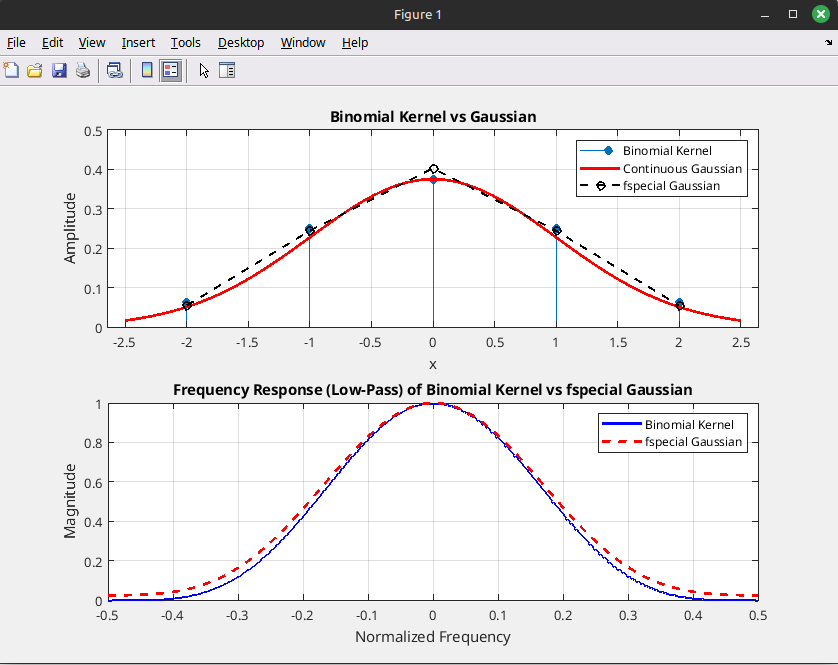
\includegraphics[width=10cm]{gaussian.png}
\caption{Plots that shows that binomial kernel approximates the gaussian filter}
\label{fig:drlagent}
\end{center}
\end{figure}




\subsection{Α2: Υλοποίηση 1D Gaussian Πυραμίδας}
\label{sec:a2}
Η Gaussian πυραμίδα δημιουργείται για 1D σήματα $x_0, x_1, \dots, x_L$ εφαρμόζοντας τις βασικές σχέσεις \eqref{eq:gaussian_kernel}–\eqref{eq:laplacian} της θεωρίας.

\paragraph{Συνέλιξη με Gaussian πυρήνα}
\mbox{}\\
Ο πυρήνας 
\[
h = \frac{1}{16}[1,4,6,4,1]^T
\]
εξομαλύνει το σήμα πριν από τη μείωση (reduce), μειώνοντας τις υψηλές συχνότητες και περιορίζοντας το aliasing (βλ. \eqref{eq:gaussian_kernel}, \eqref{eq:binomial}).

\paragraph{Downsampling (Reduce)} \mbox{} 

Διατηρούμε κάθε δεύτερο δείγμα του φιλτραρισμένου σήματος για να μειωθεί η διακριτή ανάλυση κατά 2 (βλ. \eqref{eq:reduce1}, \eqref{eq:reduce2}).

\paragraph{Toeplitz Matrix}\mbox{} 

Ο Toeplitz πίνακας χρησιμοποιείται για να υλοποιηθεί η συνέλιξη μέσω γραμμικού πολλαπλασιασμού.  
Κάθε γραμμή του πίνακα είναι μια μετατόπιση του gaussian φίλτρου.  
Ο γραμμικός συνδυασμός των στοιχείων κάθε γραμμής με τα αντίστοιχα δείγματα του σήματος δίνει το αποτέλεσμα της συνέλιξης:
\[
y = T \cdot x
\]
Αυτό αντιστοιχεί στις εξισώσεις \eqref{eq:reduce1} και \eqref{eq:reduce2}.

\paragraph{Downsampling με $D_N$}\mbox{} 

Το $D_N$ matrix επιλέγει τα δείγματα που θα κρατηθούν μετά τη συνέλιξη:  
έχει μονάδες στις θέσεις των στοιχείων που θα διατηρηθούν και μηδενικά αλλού.  
Η εφαρμογή του στο φιλτραρισμένο σήμα υλοποιεί το downsampling,
όπως περιγράφηκε παραπάνω και στις εξισώσεις \eqref{eq:reduce2}.
Στην ουσία ο $D_N$ είναι ένας γραμμικός τελεστής που μειώνει τη δειγματοληψία ενός σήματος
κατά έναν συντελεστή $N$, επιλέγοντας κάθε $N$-οστό στοιχείο, στην δικιά μας περίπτωση $N = 2$.

\paragraph{Kronecker Product}
\mbox{}\\

Στην 1D περίπτωση το γινόμενο Kronecker δεν χρησιμοποιείται άμεσα.  
Ωστόσο, σε γενικότερο πλαίσιο μπορεί να εφαρμοστεί για τη διεύρυνση του πίνακα δειγματοληψίας $D_N$ ή για 2D συνελίξεις, όπου η επεξεργασία είναι \textit{separable} κατά γραμμές και στήλες.

\subparagraph{Ορισμός}
\mbox{} \\
Αν έχουμε δύο πίνακες
\[
A \in \mathbb{R}^{m \times n}, \quad B \in \mathbb{R}^{p \times q},
\]
τότε το γινόμενο Kronecker ορίζεται ως
\[
A \otimes B,
\]
και είναι πίνακας διαστάσεων
\[
(mp) \times (nq).
\]

Ορίζεται αναλυτικά ως:
\[
A \otimes B =
\begin{bmatrix}
a_{11}B & a_{12}B & \cdots & a_{1n}B \\
a_{21}B & a_{22}B & \cdots & a_{2n}B \\
\vdots  & \vdots  & \ddots & \vdots  \\
a_{m1}B & a_{m2}B & \cdots & a_{mn}B
\end{bmatrix}
\]

Κάθε στοιχείο του πίνακα $A$ πολλαπλασιάζει ολόκληρο τον πίνακα $B$.

\subparagraph{Γιατί χρησιμοποιείται το Kronecker Product}
\mbox{} \\
Το γινόμενο Kronecker χρησιμοποιείται εκτενώς στην επεξεργασία σήματος και εικόνας διότι:

\begin{itemize}
    \item Μετατρέπει 2D πράξεις σε 1D (vectorized) μορφή.
    \item Εκφράζει φυσικά \textit{separable φίλτρα}.
    \item Απλοποιεί την ανάλυση και υλοποίηση πράξεων κατά γραμμές και στήλες.
\end{itemize}

\subparagraph{Separable Φίλτρα}

Για ένα separable φίλτρο ισχύει:
\[
H_{2D} = H_y \otimes H_x
\]
δηλαδή το 2D φίλτρο προκύπτει ως Kronecker γινόμενο δύο 1D φίλτρων, ένα για τον άξονα $x$ και ένα για τον άξονα $y$.

\subparagraph{Kronecker και Δειγματοληψία}
\mbox{} \\
Η 2D υποδειγματοληψία μπορεί να γραφτεί ως:
\[
D_{2D} = D_y \otimes D_x
\]
δηλαδή εφαρμόζεται Kronecker γινόμενο των 1D downsampling τελεστών σε κάθε άξονα.

\subparagraph{Σύνδεση με FFT}
\mbox{} \\
Στην ανάλυση συχνοτήτων:

\begin{itemize}
    \item Κάθε άξονας (γραμμές και στήλες) αναλύεται ανεξάρτητα.
    \item Το 2D FFT ισοδυναμεί με:
    \begin{itemize}
        \item FFT κατά τις γραμμές
        \item FFT κατά τις στήλες
    \end{itemize}
\end{itemize}

Για separable φίλτρο στο πεδίο συχνοτήτων ισχύει:
\[
H(\omega_x, \omega_y) = H_x(\omega_x)\, H_y(\omega_y)
\]

Δηλαδή, το 2D FFT του φίλτρου ισοδυναμεί με το γινόμενο δύο 1D FFT, ένα για κάθε άξονα.

\paragraph{Δημιουργία Gaussian Πυραμίδας}\mbox{} 

Η συνάρτηση \texttt{gaussianPyramid(x,L)} επαναλαμβάνει:
\begin{enumerate}
    \item Συνέλιξη με gaussian kernel (toeplitz) → smoothing (\eqref{eq:gaussian_kernel}, \eqref{eq:binomial})
    \item Downsampling με $D_N$ (\eqref{eq:reduce1}, \eqref{eq:reduce2})
    \item Αποθήκευση κάθε επιπέδου $x_j$ στο cell array $G\{j\}$
\end{enumerate}
Το αρχικό σήμα είναι το επίπεδο 0 ($x_0$). Κάθε επόμενο επίπεδο $x_{j+1}$ είναι πιο ομαλό και μικρότερο σε μέγεθος.

\paragraph{Εφαρμογή σε παράδειγμα 1D σήματος}\mbox{} 

Χρησιμοποιήθηκε το σήμα:
\[
x = \sin(2t) + 0.5 \sin(5t), \quad t \in [0,2\pi], \quad N=64
\]
Δημιουργήθηκαν 5 επίπεδα πυραμίδας ($x_0$ έως $x_4$).  
Ξεκινώντας από το αρχικό σήμα $x_0$, σε κάθε επίπεδο εφαρμόζεται πρώτα το φίλτρο και μετά το downsampling, σύμφωνα με τις εξισώσεις \eqref{eq:reduce1}--\eqref{eq:reduce2}. Τα αντίστοιχα plots παρατίθενται παρακάτω, περιλαμβάνοντας και το αρχικό σήμα $x_0$.


\begin{figure}[h!]
    \begin{center}
    \begin{minipage}{0.45\textwidth}
        \centering
        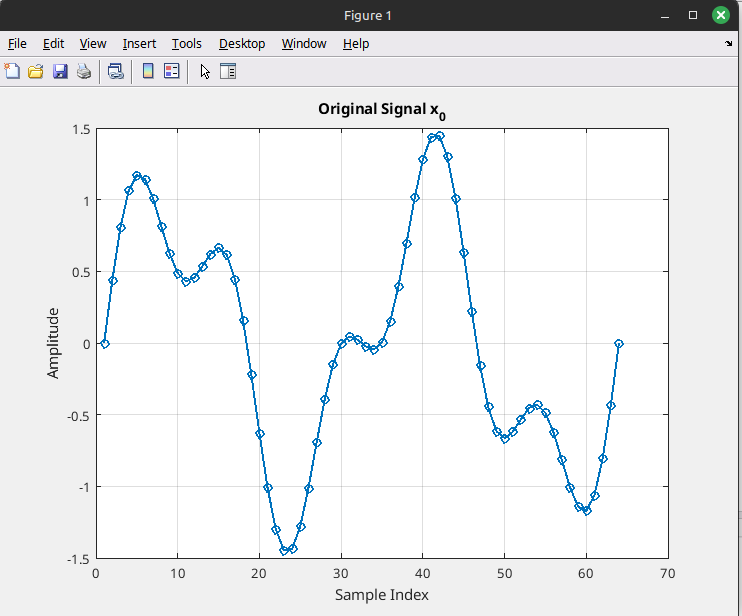
\includegraphics[width=\textwidth]{x_0.png}
        \caption{Αρχικό σήμα $x_0$}
        \label{fig:original_signal}
    \end{minipage}
    \hfill
    \begin{minipage}{0.45\textwidth}
        \centering
        
\includegraphics[width=\textwidth]{gaussian1D.png}
        \caption{Gaussian πυραμίδα 1D: κάθε επίπεδο δείχνει το σήμα μετά Gaussian φίλτρο και downsampling}
        \label{fig:gaussian_pyramid}
    \end{minipage}
    \end{center}
\end{figure}

\paragraph{Εξήγηση των Plots}\mbox{} 

Στα plots παρουσιάζονται όλα τα επίπεδα της Gaussian πυραμίδας:
\begin{itemize}
    \item \textbf{Επίπεδο 0:} Το αρχικό σήμα με όλες τις συχνότητες.
    \item \textbf{Επίπεδα 1–4:} Το σήμα γίνεται σταδιακά πιο ομαλό λόγω του gaussian φίλτρου. Η διακριτή ανάλυση μειώνεται επειδή διατηρούμε κάθε δεύτερο δείγμα.  
    Τα plots δείχνουν οπτικά τη διαδικασία smoothing και υποδειγματοληψίας, όπως περιγράφεται στις εξισώσεις \eqref{eq:reduce1}–\eqref{eq:reduce2}.
\end{itemize}

Η διαδικασία αυτή αποτελεί τη βάση για την κατασκευή laplacian πυραμίδων (\eqref{eq:gaussian_laplacian}) και τελικά την ανακατασκευή του σήματος (\eqref{eq:reconstruction}).  

Η ίδια λογική μπορεί να εφαρμοστεί σε 2D εικόνες με separable convolution: πρώτα κατά γραμμές, μετά κατά στήλες.










\subsection{A3: Από Gaussian σε Laplacian και Ανακατασκευή (1D)}
\label{sec:a3}

\subsubsection{Κατασκευή Laplacian Πυραμίδας}

Η laplacian πυραμίδα παράγεται από τα επίπεδα της γκαουσιανής πυραμίδας χρησιμοποιώντας την βασική σχέση της θεωρίας για laplacian επίπεδο (βλ. eq:\ref{eq:laplacian}), όπου η \texttt{expand} περιλαμβάνει upsampling κατά 2 και συνέλιξη με τον gaussian πυρήνα $h$ (βλ. eq:\ref{eq:expand}).  

Κάθε επίπεδο λαπλασιανής περιέχει τις λεπτομέρειες υψηλών συχνοτήτων που αφαιρέθηκαν κατά το downsampling. Το τελευταίο επίπεδο laplacian είναι απλώς το coarsest gaussian επίπεδο (βλ. eq:\ref{eq:laplacian}).

\subsubsection{Ανακατασκευή του Αρχικού Σήματος}

Η ανακατασκευή του αρχικού σήματος $G_0$ γίνεται σύμφωνα με την βασική σχέση της θεωρίας (βλ. eq:\ref{eq:reconstruction}).  

Ξεκινάμε από το πιο coarse επίπεδο $G_L$ και προσθέτουμε σταδιακά τις λεπτομέρειες από τα αντίστοιχα laplacian επίπεδα $L_j$.  
Αυτό επιβεβαιώνει ότι η laplacian πυραμίδα περιέχει όλη την απαραίτητη πληροφορία για πλήρη ανακατασκευή, καθώς κάθε επίπεδο λειτουργεί ως ζώνη συχνοτήτων (band-pass).

\subsubsection{Υλοποίηση}

\begin{itemize}
    \item \textbf{Gaussian Pyramid:} \texttt{gaussianPyramid(x,L)} – δημιουργεί όλα τα επίπεδα gaussian πυραμίδας (βλ. \ref{sec:a2}).
    \item \textbf{Expand / Upsample:} \texttt{gaussianExpand(x)} – επαναδειγματοληψία και συνέλιξη με gaussian kernel (βλ. eq:\ref{eq:expand}).
    \item \textbf{Laplacian Pyramid:} \texttt{buildLaplacianPyramid(G)} – υπολογίζει κάθε επίπεδο laplacian (βλ. eq:\ref{eq:laplacian}).
    \item \textbf{Reconstruction:} \texttt{reconstructFromLaplacian(L)} – ανακατασκευάζει το αρχικό σήμα από τη laplacian πυραμίδα και το coarsest gaussian επίπεδο (βλ. eq:\ref{eq:reconstruction}).
\end{itemize}

Ο κώδικας χρησιμοποιεί toeplitz matrices για συνέλιξη, DN matrices για downsampling και upsampling, διασφαλίζοντας την ακρίβεια της ανακατασκευής.

\bigskip
\noindent
Παρακάτω παρατίθενται τα plots για την laplacian πυραμίδα και την ανακατασκευή του σήματος (το αρχικό σήμα $x_0$ υπάρχει ήδη στο figure (βλ. fig:\ref{fig:original_signal}) όπως και η gaussian πυραμίδα (βλ. fig:\ref{fig:gaussian_pyramid})):


\begin{figure}[h!]
    \begin{center}
    \begin{minipage}{0.32\textwidth}
        \centering
        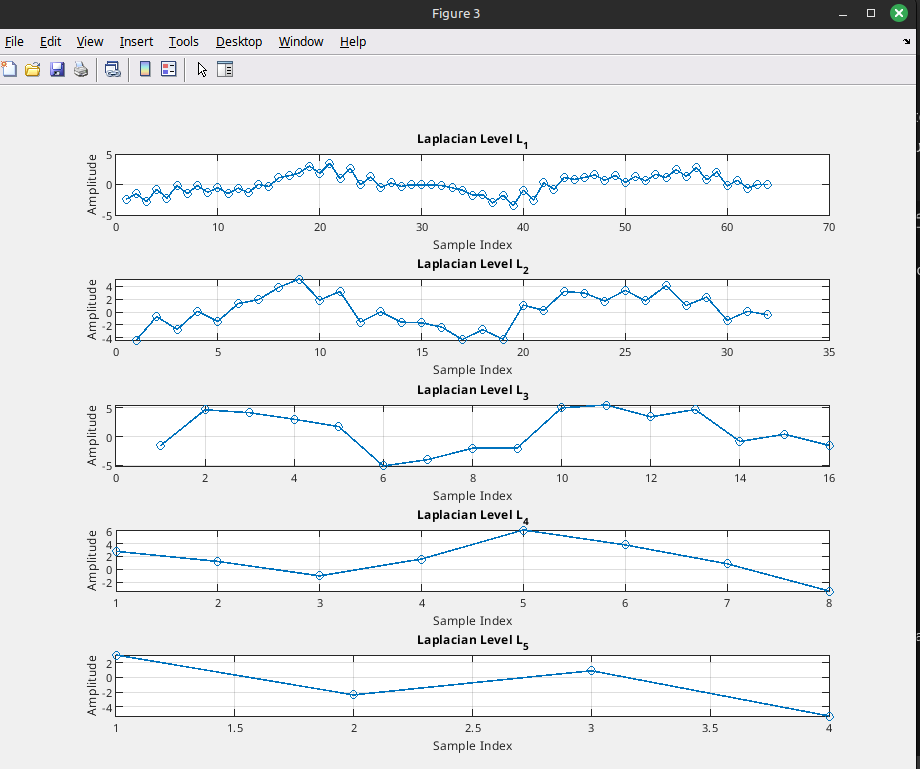
\includegraphics[width=\textwidth]{laplacianpyramid.png}
        \caption{Laplacian πυραμίδα 1D: λεπτομέρειες υψηλών συχνοτήτων}
        \label{fig:laplacian_pyramid}
    \end{minipage}
    \hfill
    \begin{minipage}{0.32\textwidth}
        \centering
        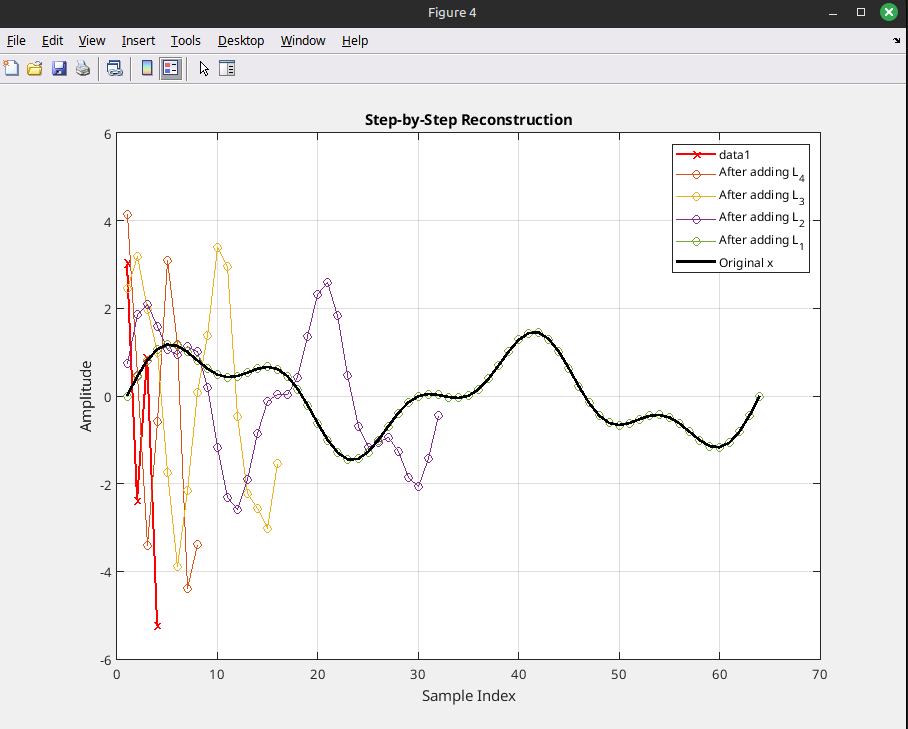
\includegraphics[width=\textwidth]{reco.png}
        \caption{Ανακατασκευή σήματος από laplacian πυραμίδα}
        \label{fig:reconstructed_signal}
    \end{minipage}
    \hfill
    \begin{minipage}{0.32\textwidth}
        \centering
        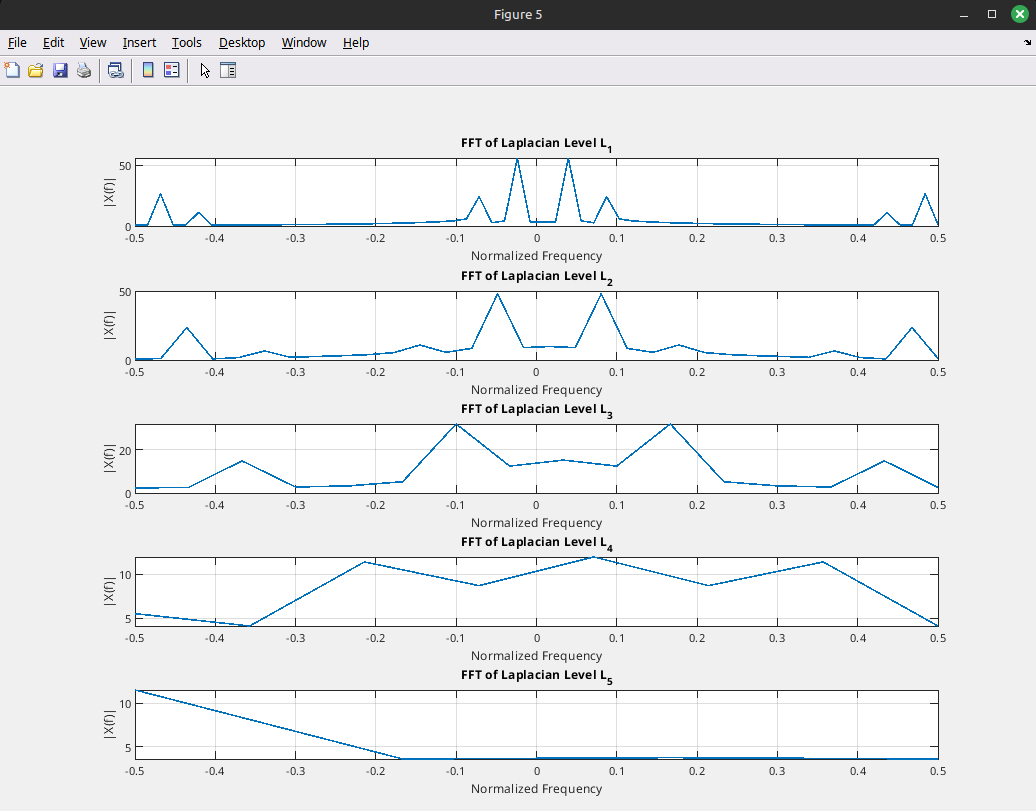
\includegraphics[width=\textwidth]{fftlaplacian.png}
        \caption{FFT των laplacian levels: band-pass στα πρώτα, low-pass residual στο τελευταίο}
        \label{fig:fft_laplacian}
    \end{minipage}
    \end{center}
\end{figure}

\subsubsection{Εξήγηση των Plots}

\begin{itemize}
    \item \textbf{Original Signal:} Το αρχικό σήμα $x_0$ εμφανίζεται ήδη στο figure (βλ. fig:\ref{fig:original_signal}).
    \item \textbf{Gaussian Pyramid:} Κάθε επίπεδο δημιουργείται με gaussian φίλτρο και downsampling (βλ. \ref{sec:a2}, eq:\ref{eq:reduce1}, eq:\ref{eq:reduce2}). Παρατηρείται σταδιακή μείωση λεπτομέρειας, με το τελευταίο επίπεδο να περιέχει μόνο χαμηλές συχνότητες.
    \item \textbf{Laplacian Pyramid:} Αναπαριστά τις λεπτομέρειες που αφαιρούνται σε κάθε στάδιο της gaussian πυραμίδας. Τα πρώτα επίπεδα περιέχουν υψηλές συχνότητες, ενώ το τελευταίο επίπεδο διατηρεί μόνο τις βασικές χαμηλές συχνότητες (βλ. eq:\ref{eq:laplacian}).
    \item \textbf{Reconstruction:} Το σήμα ανακατασκευάζεται ξεκινώντας από το πιο coarse επίπεδο. Κάθε στάδιο προσθέτει τις λεπτομέρειες υψηλών συχνοτήτων από την laplacian πυραμίδα, μέχρι να φτάσουμε στο αρχικό σήμα $x_0$ (βλ. eq:\ref{eq:laplacian_gaussian}, eq:\ref{eq:reconstruction}).
    \item \textbf{FFT των Laplacian Levels:} Στο plot των ftt των laplacian levels βλέπουμε ότι τα πρώτα επίπεδα $L_1,L_2,\dots,L_{end-1}$ είναι band-pass, με μηδενική σχεδόν ενέργεια γύρω από $f = 0$ και κορυφές σε ενδιάμεσες συχνότητες που μετατοπίζονται προς χαμηλότερες συχνότητες όσο προχωράμε στα βαθύτερα επίπεδα, ενώ το τελευταίο επίπεδο $L_{end}$ κρατάει τις πολύ χαμηλές συχνότητες ως low-pass residual. Αυτό δείχνει ότι κάθε επίπεδο αντιστοιχεί σε διαφορετική ζώνη συχνοτήτων.
\end{itemize}











\subsection{A4 — Μελέτη Toolbox Πυραμίδων MATLAB}

Η toolbox πυραμίδων του MATLAB  \url{https://www.mathworks.com/matlabcentral/fileexchange/30790-image-pyramid-gaussian-and-laplacian}
 προσφέρει εργαλεία για τη δημιουργία gaussian και laplacian πυραμίδων, καθώς και για blending, τα οποία υλοποιούν άμεσα τις θεωρητικές αρχές που παρουσιάστηκαν στα \ref{sec:a2},\ref{sec:a3}.
Οι κύριες συναρτήσεις είναι οι εξής:

\begin{enumerate}
    \item \textbf{gen\_Pyr()}: Δημιουργεί την gaussian ή laplacian πυραμίδα ενός σήματος ή εικόνας.  
    Κάνει διαδοχικές κλήσεις στη \texttt{pyr\_Reduce} για όλα τα επίπεδα και παρέχει μια πλήρη αναπαράσταση του σήματος σε πολλαπλές κλίμακες.

    \item \textbf{pyr\_Reduce()}: Εκτελεί συνέλιξη με Gaussian kernel και downsampling. Υλοποιεί τις πράξεις reduce που περιγράφονται στις σχέσεις (\eqref{eq:reduce1}, \eqref{eq:reduce2}, \eqref{eq:reduce_expand})  και μειώνει  το μέγεθος κάθε επιπέδου, διατηρώντας χαμηλές συχνότητες.

    \item \textbf{pyr\_Expand()}:  Εκτελεί upsampling ενός επιπέδου και συνέλιξη με Gaussian kernel (\eqref{eq:expand}),
    κλιμακώνοντας τους συντελεστές του φίλτρου ώστε να διατηρείται η συνολική ενέργεια, όπως στο παράδειγμα 1D (βλ. \ref{sec:a2}). 

    \item \textbf{pyrBlend()}: Συνδυάζει δύο laplacian πυραμίδες χρησιμοποιώντας gaussian μάσκα σε κάθε επίπεδο (\eqref{eq:blending}, \eqref{eq:blended_reconstruction}). 

    \item \textbf{pyr\_Reconstruct()}: Ανακατασκευάζει το αρχικό σήμα ή εικόνα από laplacian πυραμίδα και το coarsest gaussian επίπεδο.  
    Υλοποιεί την ανακατασκευή από laplacian σε gaussian (\eqref{eq:laplacian_gaussian}, \eqref{eq:reconstruction}) και επιβεβαιώνει ότι η πυραμίδα διατηρεί όλες τις απαραίτητες λεπτομέρειες για πλήρη ανακατασκευή.
\end{enumerate}



\section{Μέρος Β — Image Blending \&  Συρραφή} 
\subsection{B1. Συρραφή apple.jpg \&  orange.jpg}

\subsubsection*{1. Feathered Mask}

\textbf{Σκοπός:} Δημιουργία ομαλής μετάβασης ανάμεσα στις δύο εικόνες.
\mbox{}\\
\textbf{Λειτουργία:} Αριστερά λευκή (apple), δεξιά μαύρη (orange), με gaussian blur για smooth blending.


\subsubsection{2. Gaussian Pyramid της μάσκας}

\textbf{Σκοπός:} Ανάλυση της μάσκας σε διαφορετικές κλίμακες για σταδιακό blending.
\mbox{}\\
\textbf{Λειτουργία:} Με κάθε επίπεδο η ανάλυση μειώνεται και οι λεπτομέρειες θολώνουν.
\mbox{}\\
\textbf{Plotting:} 
\begin{itemize}
    \item Level 1: Σχεδόν ίδια με την αρχική μάσκα, υψηλή ανάλυση, καθαρά όρια.
    \item Level 2-4: Σταδιακά πιο θολά, το κέντρο της μετάβασης γίνεται πιο ευρύ, smoother transition.
    \item Level 5: Πολύ θολό, εμφανίζεται μόνο το γενικό σχήμα, χαμηλές συχνότητες χωρίς λεπτομέρειες.
    \item Η αρχική μάσκα εμφανίζεται με σταδιακή μετάβαση από λευκό σε μαύρο, δείχνοντας πώς η περιοχή μετάβασης είναι εξομαλυμένη. Αυτό εξηγεί γιατί η τελική εικόνα δεν έχει απότομες ακμές στην περιοχή που συναντώνται οι δύο εικόνες.

\end{itemize}

\begin{figure}[h!]
\centering
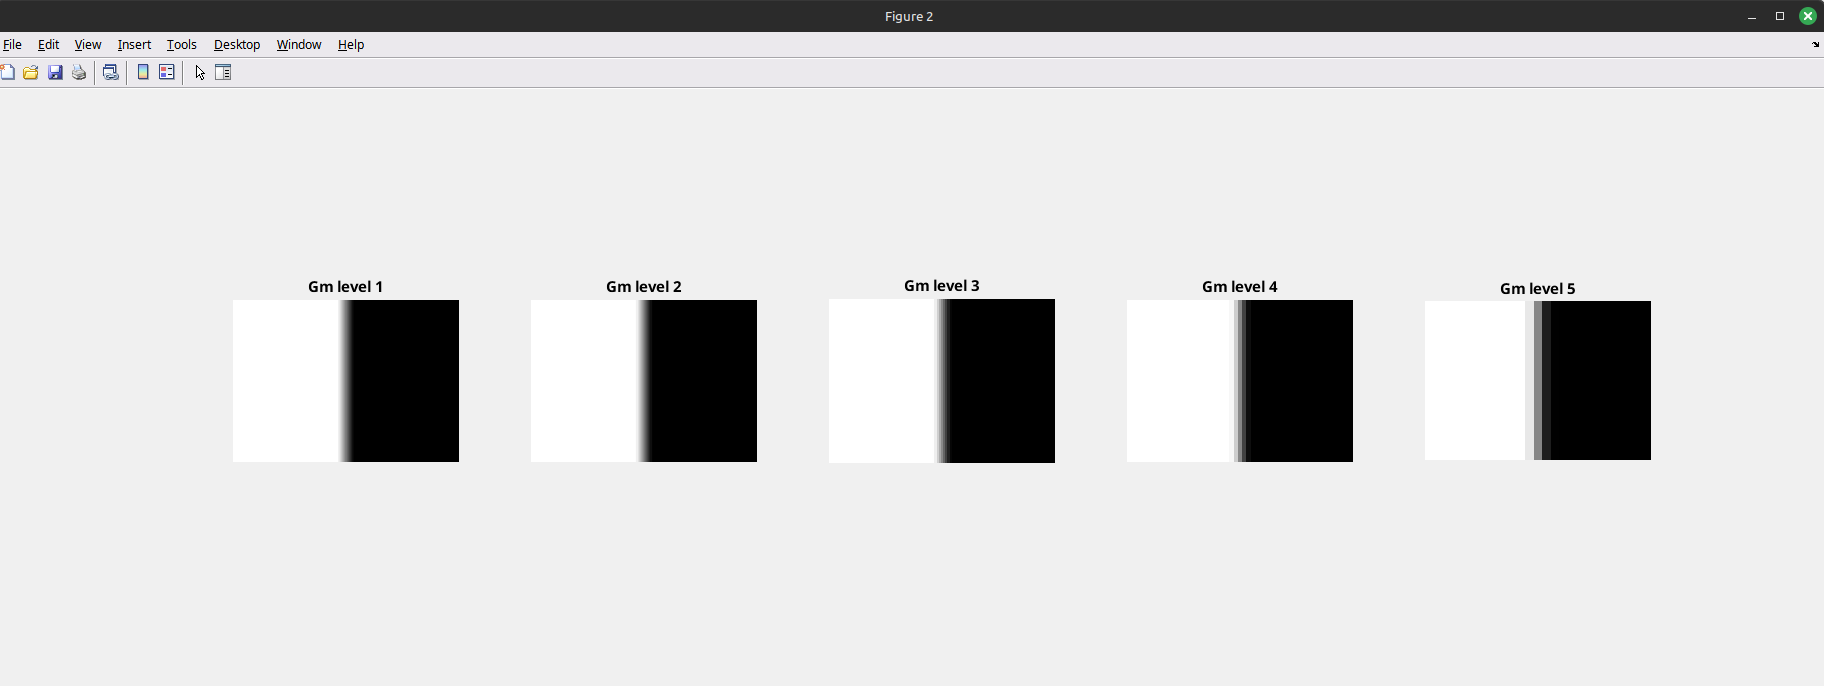
\includegraphics[width=0.6\textwidth]{gaussian_mask.png}
\caption{Gaussian πυραμίδα της μάσκας}
\label{fig:mask_gaussian_pyramid}
\end{figure}

\subsubsection{3. Laplacian Pyramid των εικόνων }

\textbf{Σκοπός:} Διαχωρισμός των εικόνων σε επίπεδα συχνοτήτων ώστε να συνδυάζονται λεπτομέρειες και γενικές μορφές ξεχωριστά.
\mbox{}\\
\textbf{Λειτουργία:}
\begin{itemize}
    \item Χαμηλές συχνότητες → συνολική φωτεινότητα και σχήμα
    \item Υψηλές συχνότητες → λεπτομέρειες και ακμές
\end{itemize}
\mbox{}\\
\textbf{Plotting (apple):}
\begin{itemize}
    \item Level 1: Υψηλή ανάλυση, εμφανείς λεπτομέρειες (φλούδα, σκιές)
    \item Level 2-4: Σταδιακά πιο θολά, λιγότερες λεπτομέρειες, κυριαρχούν οι χαμηλές συχνότητες
    \item Level 5: Πολύ θολό, μόνο γενικό σχήμα της apple, υψηλή ένταση φωτεινότητας λόγω gaussian τελευταίου επιπέδου
\end{itemize}

Αντίστοιχα, η laplacian pyramid της orange εμφανίζει τις λεπτομέρειες και τη δομή σε διαφορετικές κλίμακες.

\begin{figure}[h!]
\centering
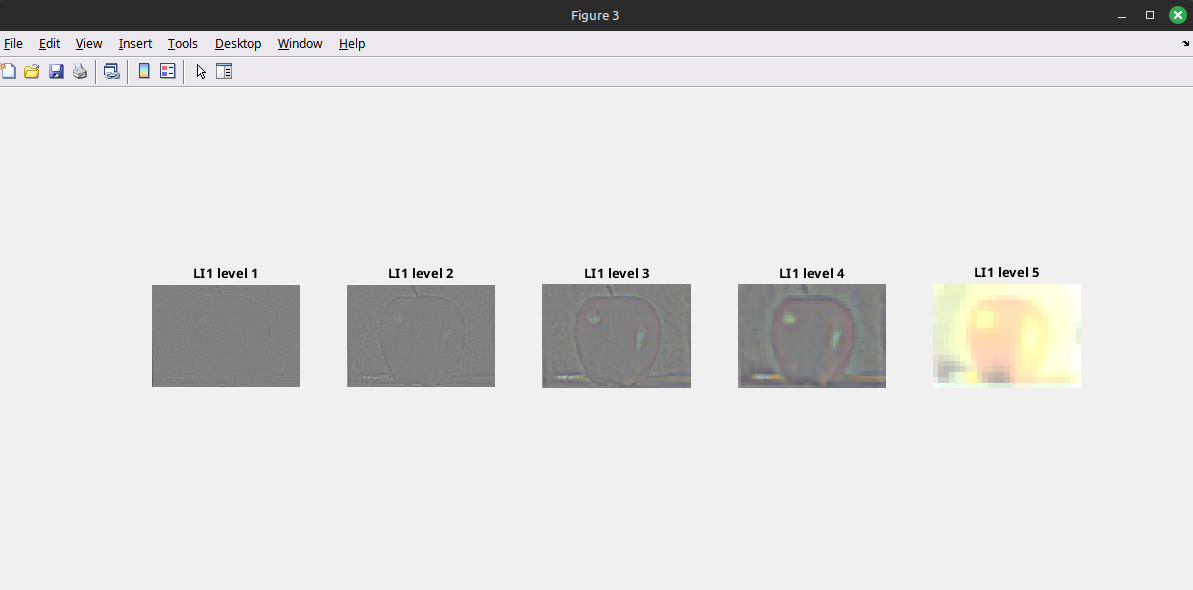
\includegraphics[width=0.8\textwidth]{LI1.png}
\caption{Laplacian πυραμίδες της εικόνας apple}
\label{fig:laplacian_pyramids}
\end{figure}

\subsubsection{4. Blended Pyramid (B)}

\textbf{Σκοπός:} Συνδυασμός των laplacian πυραμίδων των δύο εικόνων βάσει της gaussian μάσκας για κάθε επίπεδο.
\mbox{}\\
\textbf{Λειτουργία:}
\[
B_i = G_i \cdot L_{Apple,i} + (1 - G_i) \cdot L_{Orange,i}
\]
όπως αναφέρθηκε και σην σχέση \ref{eq:blending}, όπου $G_i$ είναι το i-οστό επίπεδο της gaussian μάσκας, και $L_{Apple,i}$, $L_{Orange,i}$ τα αντίστοιχα επίπεδα laplacian των εικόνων apple και orange.
\mbox{}\\
\textbf{Plotting:} 
\begin{itemize}
    \item Επίπεδο 1–2 (Υψηλή ανάλυση): Οι λεπτές λεπτομέρειες και υφές και από τις δύο εικόνες είναι ορατές. Οι άκρες αναμειγνύονται σύμφωνα με τη μάσκα gauss, δείχνοντας αρχική ομαλή μετάβαση.
    \item Επίπεδο 3–4 (Ενδιάμεση ανάλυση): Οι λεπτομέρειες σταδιακά θολώνουν. Οι άκρες μαλακώνουν και η μάσκα δημιουργεί ένα πιο ομοιογενές μείγμα μεταξύ apple και orange.
    \item Επίπεδο 5 (Χαμηλή ανάλυση): Μόνο τα γενικά σχήματα παραμένουν. Οι λεπτές υφές εξαφανίζονται, αφήνοντας μια ομαλή συνολική μετάβαση που διασφαλίζει ότι η τελική ανακατασκευασμένη εικόνα φαίνεται "φυσική".

\end{itemize}

\newpage
\begin{figure}[h!]
\centering
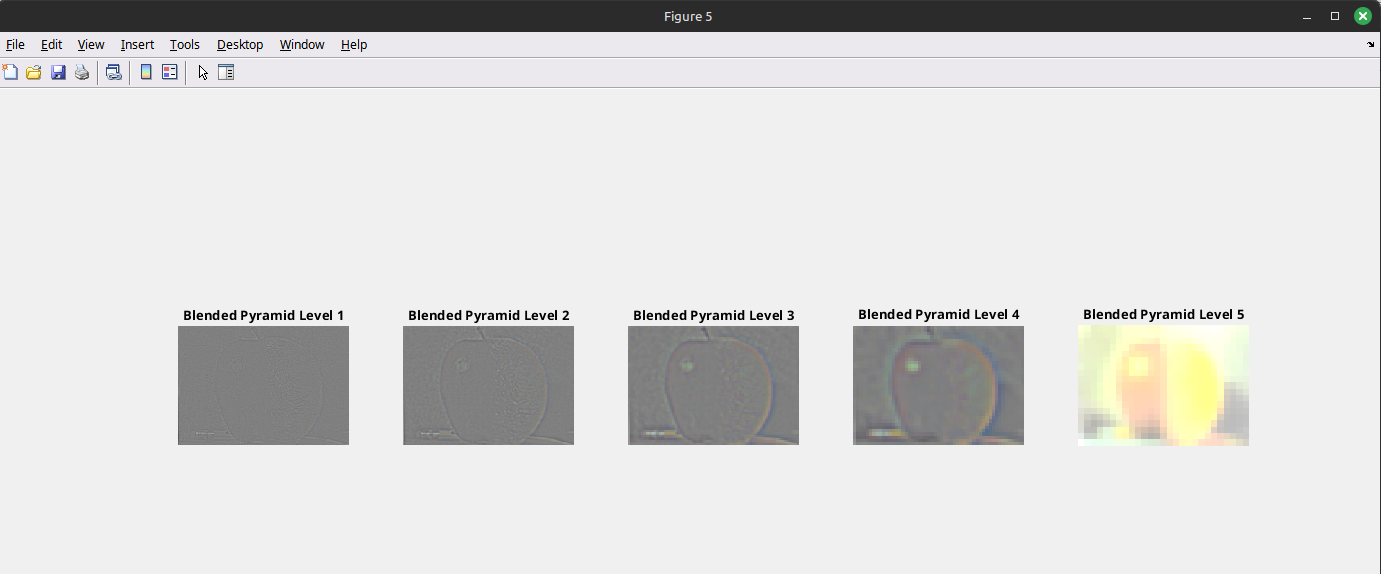
\includegraphics[width=0.8\textwidth]{blended_pyramid.png}
\caption{Blended pyramid: συνδυασμός laplacian πυραμίδων βάσει της gaussian μάσκας}
\label{fig:blended_pyramid}
\end{figure}

\subsubsection{5. Ανακατασκευή τελικής εικόνας}

\textbf{Σκοπός:} Σύνθεση όλων των επιπέδων της blended pyramid σε μία τελική εικόνα.
\mbox{}\\
\textbf{Λειτουργία:} Οι λεπτομέρειες από τα χαμηλά επίπεδα και η γενική δομή από τα υψηλά επίπεδα συνδυάζονται με smooth transition χάρη στη μάσκα.
\mbox{}\\
\textbf{Plotting:} Η τελική blended εικόνα δείχνει ομαλή σύνδεση μεταξύ apple  και orange, χωρίς απότομες αλλαγές, με φυσικό gradient στη μέση.
\mbox{}\\
\newpage
\begin{figure}[h!]
\centering
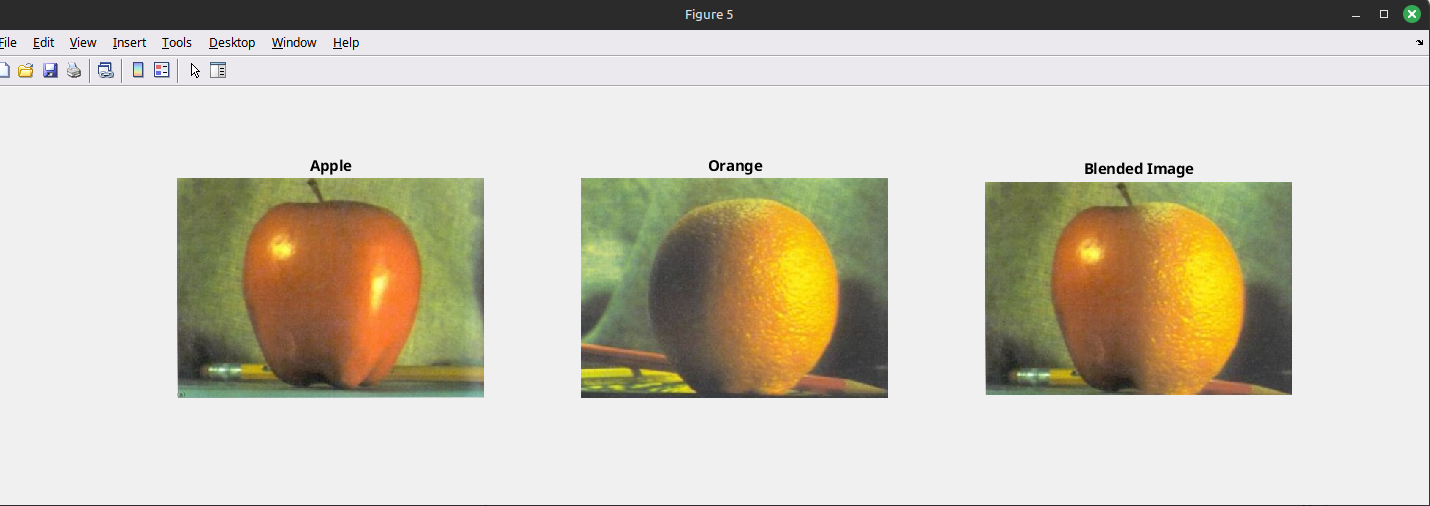
\includegraphics[width=0.7\textwidth]{blended.png}
\caption{Σύγκριση αρχικών εικόνων και τελικής blended εικόνας}
\label{fig:blended}
\end{figure}

\subsection{Συρραφή woman.png \&  hand.png}

\subsubsection{1. Επιλογή μάσκας}
Η μάσκα δημιουργήθηκε με τη συνάρτηση \texttt{drawfreehand} πάνω στην εικόνα της γυναίκας και χρησιμοποιήθηκε ως αρχική μάσκα $M_0$ για την κατασκευή γκαουσιανής πυραμίδας μάσκας.  
Η επιλογή επικεντρώθηκε στην περιοχή του ματιού, ώστε αυτό να διατηρηθεί καθαρό στο τελικό αποτέλεσμα, ενώ οι γύρω περιοχές (π.χ. υπόλοιπο πρόσωπο, μαλλιά) αποφεύχθηκαν για να μην επηρεάσουν τη διαδικασία blending.

Η αρχική μάσκα εξομαλύνθηκε μέσω διαδοχικών gaussian φιλτραρισμάτων και μειώσεων ανάλυσης (βλ. eq: \ref{eq:gaussian_kernel}, eq: \ref{eq:reduce1}), ώστε να παραχθούν τα επίπεδα $G^M_j$ της gaussian πυραμίδας της μάσκας.  
Με τον τρόπο αυτό αποφεύγονται απότομες μεταβάσεις και εξασφαλίζεται ομαλή κατανομή βαρών κατά τη διαδικασία blending.

\subsubsection{2. Επίδραση της μάσκας και blending}
Η διαδικασία blending πραγματοποιήθηκε σε κάθε επίπεδο της λαπλασιανής πυραμίδας σύμφωνα με τη σχέση:
\begin{equation}
B_j = G^M_j \odot L^A_j + (1 - G^M_j) \odot L^B_j
\end{equation}
όπως ορίζεται στην εξίσωση \eqref{eq:blending}.




\begin{itemize}
    \item Η gaussian πυραμίδα της μάσκας εξασφαλίζει ομαλές μεταβάσεις μεταξύ των δύο εικόνων σε διαφορετικές κλίμακες ανάλυσης.
    \item Στις περιοχές όπου η μάσκα λαμβάνει υψηλές τιμές ($G^M_j \approx 1$), κυριαρχούν τα laplacian επίπεδα της εικόνας \texttt{woman}, διατηρώντας καθαρά τα χαρακτηριστικά του ματιού.
    \item Στις περιοχές με χαμηλές τιμές μάσκας ($G^M_j \approx 0$), υπερισχύουν τα laplacian επίπεδα της εικόνας \texttt{hand}, αναδεικνύοντας τις λεπτομέρειες του χεριού.
\end{itemize}

Τα χαμηλά επίπεδα της laplacian πυραμίδας (υψηλές συχνότητες) συνεισφέρουν κυρίως στις λεπτομέρειες του χεριού, ενώ τα υψηλότερα επίπεδα (χαμηλές συχνότητες) διατηρούν τη συνολική φωτεινότητα και τα βασικά χαρακτηριστικά του ματιού.
Οι περιοχές εκτός της μάσκας του ματιού εμφανίζονται περισσότερο σαν το χέρι, καθώς η εικόνα \texttt{hand} κυριαρχεί μέσω του όρου $(1 - G^M_j)$.


\subsubsection{3. Feathered edge blending \&  Ανακατασκευή τελικής εικόνας}
Μετά την ανακατασκευή της blended εικόνας, εφαρμόστηκε feathered edge blending: η αρχική μάσκα θολώθηκε με γκαουσιανό φίλτρο για να μαλακώσουν οι άκρες και επεκτάθηκε σε 3 κανάλια για ομοιόμορφο blending για να διατηρηθεί το makeup στο μάτι. Επίσης το μάτι της γυναίκας συγχωνεύτηκε φυσικά στο κέντρο του χεριού χωρίς εμφανή όρια ή σκιές. Η τελική εικόνα προέκυψε μέσω ανακατασκευής της laplacian πυραμίδας με διαδοχικό upsampling και πρόσθεση των επιπέδων, διατηρώντας τις λεπτομέρειες του ματιού και ενσωματώνοντας ομαλά τις λεπτομέρειες του χεριού, προσφέροντας αποτέλεσμα χωρίς artifacts.
\mbox{}\\
\textbf{Plotting:} 
\mbox{}\\
Το μάτι της γυναίκας βρίσκεται στο κέντρο του χεριού, ενώ οι υπόλοιπες περιοχές του χεριού παραμένουν κυρίαρχες εκτός της μάσκας, λόγω της χωρικής κατανομής βαρών της gaussian μάσκας που περιορίζει τη συμβολή της εικόνας μόνο στο μάτι, ενώ οι ομαλές άκρες του feathered edge blending εξασφαλίζουν ενσωμάτωση χωρίς artifacts.
\begin{figure}[h!]
    \centering
    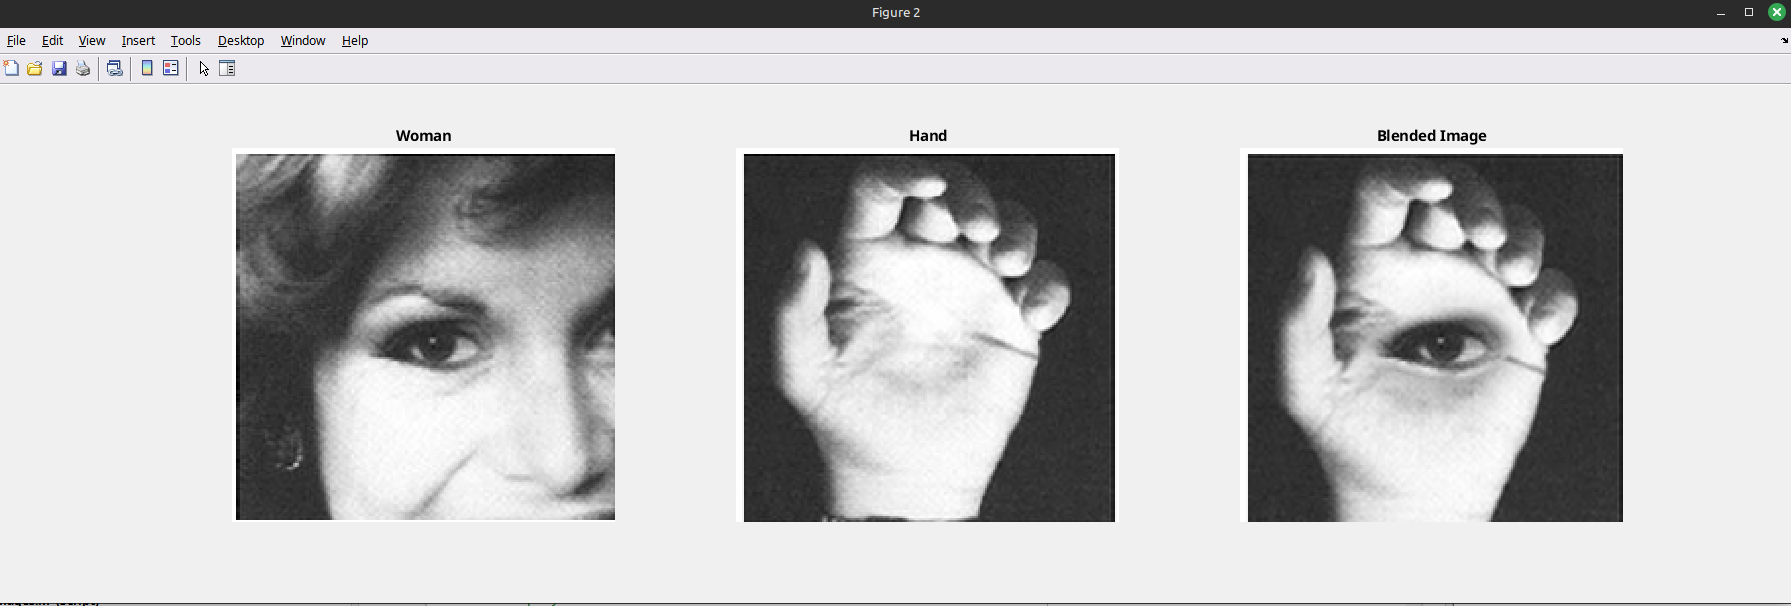
\includegraphics[width=0.7\textwidth]{woman_hand.png}
    \caption{Σύγκριση αρχικών εικόνων και τελικής blended εικόνας}
    \label{fig:woman_hand}
    \end{figure}
    

\subsection{Δημιουργία Σύνθεσης πολλών εικόνων}
Η σύνθεση πολλαπλών εικόνων αντιμετωπίζεται ως γενίκευση του blending δύο εικόνων.
\subsubsection{Επιλογή και τοποθέτηση αντικειμένων}
Η βάση της σύνθεσης είναι η εικόνα P200.jpg, που χρησιμοποιείται ως φόντο.
Τα αντικείμενα (dog1, dog2, cat, bench, mycat) τοποθετούνται σε διαφορετικά σημεία πάνω στο φόντο, ώστε να μην επικαλύπτονται

\begin{table}[h!]
    \centering
    \begin{tabular}{l l l}
    \textbf{Αντικείμενο} & \textbf{Θέση} & \textbf{Μέγεθος} \\
    dog1 & κάτω αριστερά & 0.11× \\
    dog2 & κάτω δεξιά & 0.21× \\
    cat & κάτω μέση & 0.10× \\
    bench & κέντρο & 0.34× \\
    mycat & πάνω αριστερά & 0.45× \\
    \end{tabular}
    \caption{Τοποθέτηση αντικειμένων στο φόντο με offsets και scaling}
    \label{tab:objects}
    \end{table}

\subsubsection{Δημιουργία μασκών και ιδιότητες}
Το άθροισμα όλων των μασκών σε κάθε pixel ισούται με 1:
\[
\sum_{k=1}^{6} m_k(x,y) = 1, \quad \forall (x,y)
\]
Δηλαδή, το άθροισμα όλων των μασκών σε κάθε pixel ισούται με 1, ώστε το blending να γίνεται σωστά.

\paragraph{Ιδιότητα 2 (local support)}
\mbox{}\\
Η μάσκα $m_k(x,y)$ έχει τιμή 1 μόνο στις περιοχές όπου η εικόνα $k$ είναι ενεργή:
\[
m_k(x,y) = 1 \quad \text{μόνο στις περιοχές όπου η εικόνα $k$ είναι ενεργή.}
\]
Στις υπόλοιπες περιοχές η μάσκα παίρνει τιμή 0 και τα υπόλοιπα αντικείμενα ή το φόντο καλύπτουν το pixel.

\paragraph{Smooth Blending}
\mbox{}\\
Οι μάσκες φιλτράρονται με gaussian φίλτρο για να αποφευχθούν σκληρές ακμές κατά το blending.

\paragraph{Φόντο ως ξεχωριστό αντικείμενο}
\mbox{}\\
Η μάσκα του φόντου $G_{\text{bg},j}^M$ ορίζεται ώστε να αφαιρεί τις περιοχές που καλύπτονται από τα αντικείμενα:
\[
G_{\text{bg},j}^M = 1 - \sum_{k=1}^{5} G_{k,j}^M
\]
Έτσι, το φόντο εμφανίζεται μόνο στις περιοχές που δεν καλύπτονται από άλλα αντικείμενα.

\subsubsection{Δημιουργία πυραμίδων και blending}
\paragraph{Gaussian πυραμίδες μασκών}
\mbox{}\\
Κάθε μάσκα υποβάλλεται σε Gaussian πυραμίδα ώστε η συμβολή κάθε αντικειμένου να μειώνεται σταδιακά στις άκρες του.

\paragraph{Laplacian πυραμίδες εικόνων}
\mbox{}\\
Κάθε εικόνα χωρίζεται σε διαφορετικές κλίμακες:
\begin{itemize}
    \item \textbf{Χαμηλά επίπεδα:} λεπτομέρειες αντικειμένων.
    \item \textbf{Ψηλά επίπεδα:} βασική φωτεινότητα και σχήμα.
\end{itemize}

\paragraph{Blending pyramid $B$}
\mbox{}\\
Για κάθε επίπεδο $j$ της πυραμίδας, το blended επίπεδο ορίζεται ως:
\[
B_j = \sum_{k=1}^{5} G^M_{k,j} \cdot L_{k,j} + G^M_{\text{bg},j} \cdot L_{\text{bg},j}
\]

όπου:

\begin{itemize}
    \item $G^M_{k,j}$ = Gaussian επίπεδο μάσκας για τα 5 αντικείμενα
    \item $L_{k,j}$ = Laplacian επίπεδο της εικόνας $k$
    \item $G^M_{\text{bg},j} = 1 - \sum_{k=1}^{5} G^M_{k,j}$ = μάσκα φόντου
    \item $L_{\text{bg},j}$ = Laplacian επίπεδο φόντου
\end{itemize}

\paragraph{Reconstruction}
\mbox{}\\
Η τελική εικόνα ανακατασκευάζεται από τα επίπεδα της blended πυραμίδας μέσω επαναλαμβανόμενης επέκτασης  και πρόσθεσης. 
Το αποτέλεσμα είναι ένα ολικό composite image, όπου κάθε αντικείμενο εμφανίζεται αποκλειστικά στις περιοχές που ορίζει η αντίστοιχη μάσκα του, με ομαλές μεταβάσεις μεταξύ αντικειμένων και φόντου.


\textbf{Plotting:} 
\mbox{}\\
Παρότι το blending είναι ομαλό σε πολυκλιμακωτό επίπεδο, ορισμένα αντικείμενα δεν ενσωματώνονται πλήρως με φυσικό τρόπο στο φόντο. Αυτό οφείλεται κυρίως σε διαφορές φωτισμού, contrast και χρωματικής κατανομής μεταξύ των επιμέρους εικόνων, καθώς και στην απουσία σκιών . Η μέθοδος blending εξαλείφει τις απότομες μεταβάσεις, αλλά δεν διορθώνει φωτομετρικές ασυνέπειες.
Το πρώτο επίπεδο της laplacian πυραμίδας εμφανίζεται σχεδόν σκοτεινό, καθώς περιέχει μόνο υψηλής συχνότητας πληροφορία (λεπτές ακμές και μικρές διαφορές έντασης). Παρότι δεν είναι οπτικά έντονο, συμβάλλει ουσιαστικά στη διατήρηση της οξύτητας και των λεπτομερειών κατά την ανακατασκευή της τελικής εικόνας.
Συνολικά, η τελική σύνθεση επιτυγχάνει συνεπές blending πολλαπλών αντικειμένων, όπως φαίνεται παρακάτω .

\begin{figure}[h!]
    \centering
    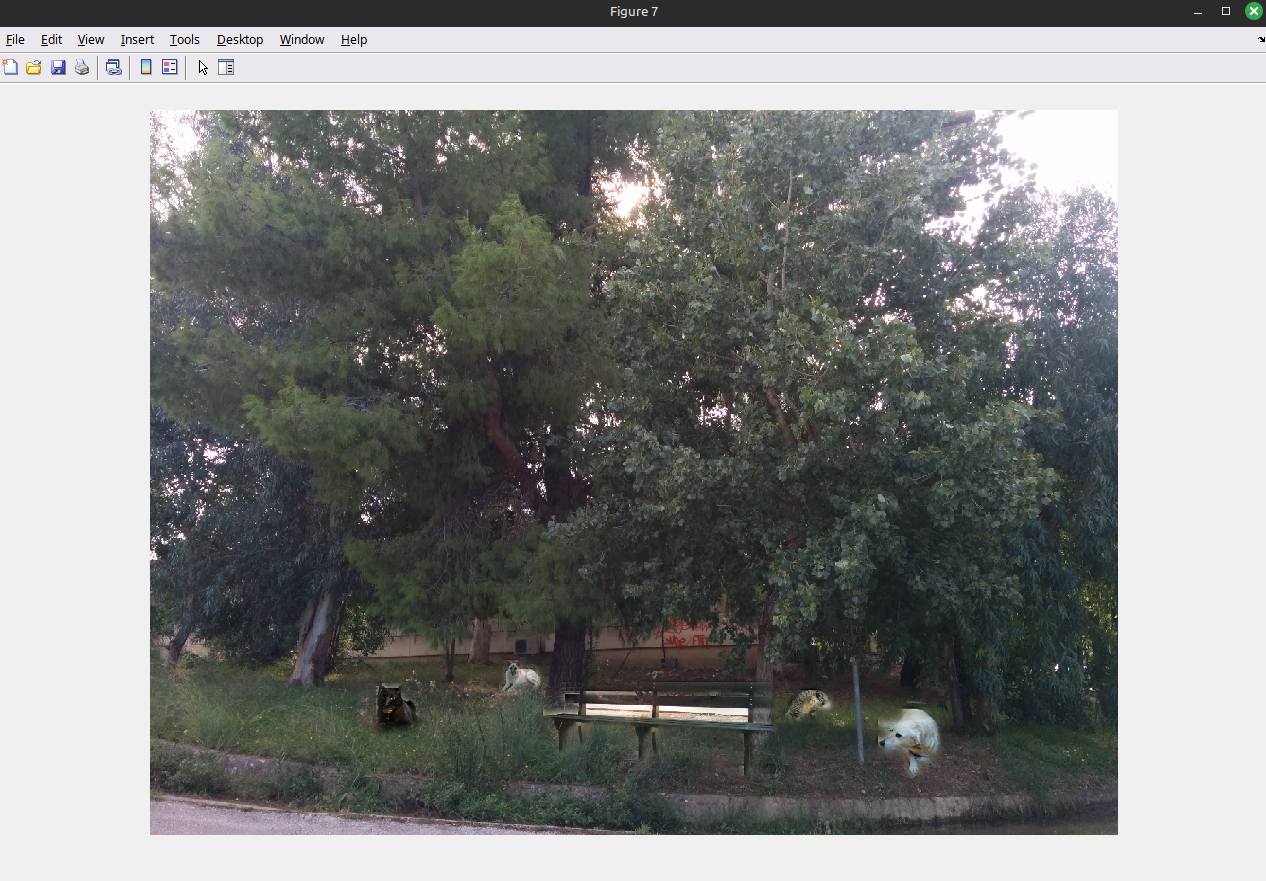
\includegraphics[width=0.59\textwidth]{6images.png}
    \caption{Συρραφή 6 εικόνων με πολυκλιμακωτό blending}
    \label{fig:6_images}
    \end{figure}


    \section{Μέρος Δ — PSPNet: Semantic Segmentation Evaluation}
    Στόχος είναι να αξιολογήσουμε ένα εκπαιδευμένο PSPNet μοντέλο πάνω στο validation dataset \textit{Cityscapes} και να υπολογίσουμε μετρικές επίδοσης κατάτμησης.
    
    \subsection{Τι είναι το Semantic Segmentation}
    Το \textit{Semantic Segmentation} είναι η διαδικασία κατά την οποία κάθε pixel μιας εικόνας ταξινομείται σε μια κατηγορία, όπως δρόμος, αυτοκίνητο, άνθρωπος ή κτίριο.  
    Διαφέρει από την απλή ταξινόμηση εικόνας γιατί αντί να βγάζει μια μόνο ετικέτα για ολόκληρη την εικόνα, δίνει ετικέτα σε κάθε pixel.
    
    \paragraph{Έξοδος:}   \mbox{}\\Feature map \(H \times W \times C\) (Height × Width × Classes)  
    Κάθε pixel παίρνει πιθανότητες για κάθε κλάση και η πρόβλεψη γίνεται ως:
    \[
    \hat{y}^{i,j} = \arg\max_c P(y_{i,j} = c)
    \]
    
    \paragraph{Είσοδος:}   \mbox{}\\εικόνα \(I \in \mathbb{R}^{H \times W \times 3}\)  
    \paragraph{Έξοδος:}   \mbox{}\\μάσκα \(\hat{Y} \in \{0,1,\dots,C-1\}^{H \times W}\) με \(C=35\)
    
    \paragraph{Εκπαίδευση:}  \mbox{}\\ Cross-Entropy Loss ανά pixel:
    \[
    \mathcal{L} = - \frac{1}{H \cdot W} \sum_{h=1}^{H} \sum_{w=1}^{W} \log \hat{Y}^{h,w}_{Y_{h,w}}
    \]
    
    \subsection{Dataset: Cityscapes}
    Το \textit{Cityscapes} χρησιμοποιείται για αστικό περιβάλλον:
    \begin{itemize}
        \item Διαστάσεις εικόνων: \(2048 \times 1024\) pixels
        \item Περιοχή: αστικά τοπία
        \item Κλάσεις: 35 
    \end{itemize}
    
    Κάθε εικόνα περιλαμβάνει:
    \begin{itemize}
        \item RGB εικόνα
        \item Ground truth mask: κάθε pixel = αριθμός κλάσης (0–34)
    \end{itemize}
    
    \subsection{Τι είναι το PSPNet (Pyramid Scene Parsing Network)}
    Το PSPNet είναι ένα βαθύ νευρωνικό δίκτυο σχεδιασμένο ειδικά για semantic segmentation που βασίζεται στην Pyramid Pooling Module (PPM).
    \paragraph{Spatial Pyramid Pooling (SPP)}
    \mbox{}\\
    \begin{itemize}
        \item Λύνει το πρόβλημα του σταθερού μεγέθους εισόδου στα CNN.
        \item Δέχεται feature map από τα προηγούμενα συνελικτικά επίπεδα και εφαρμόζει pooling σε διαφορετικά grids (π.χ., \(1\times1, 2\times2, 3\times3, 6\times6\) bins).
        \item Κωδικοποιεί χωρική πληροφορία σε πολλαπλές κλίμακες χωρίς να χρειάζεται να αλλάξεις το μέγεθος εισόδου εικόνας.
    \end{itemize}
    
    \paragraph{Pyramid Pooling Module (PPM)}
    \mbox{}\\
    Το PPM βοηθά το δίκτυο να βλέπει τόσο ολόκληρη τη σκηνή όσο και λεπτομέρειες:
    \begin{itemize}
        \item Παίρνει τα features maps από το CNN backbone.
        \item Κάνει pooling σε διαφορετικά επίπεδα .
        \item Συνενώνει όλα τα pooled maps με concatenation:
        \[
        F_l = \text{Pooling}_{n_l \times n_l}(F), \quad F_\text{concat} = \text{Concat}(F_1, F_2, \dots, F_L)
        \]
    \end{itemize}
    
    Με αυτό τον τρόπο, το PSPNet:
    \begin{itemize}
        \item Βλέπει global context (π.χ. ολόκληρος δρόμος)
        \item Κρατά local λεπτομέρειες (π.χ. άνθρωποι, πινακίδες)
        \item Ανιχνεύει αντικείμενα διαφορετικών μεγεθών
    \end{itemize}
    
    \subsection{Μετρικές Αξιολόγησης}
    \mbox{}\\
    \paragraph{Intersection over Union (IoU)}
    Μετράει πόσο καλά η πρόβλεψη επικαλύπτεται με την πραγματική μάσκα για κάθε κλάση:
    \[
    \text{IoU}_c = \frac{|\text{Prediction}_c \cap \text{GT}_c|}{|\text{Prediction}_c \cup \text{GT}_c|}
    \]
    
    \paragraph{Σημαντικές παρατηρήσεις:}
    \mbox{}\\
    \begin{itemize}
        \item \(\text{Prediction}_c\): pixels που προβλέφθηκαν ως κλάση \(c\)
        \item \(\text{GT}_c\): pixels που πραγματικά ανήκουν στην κλάση \(c\)
        \item Όσο πιο κοντά στο 1, τόσο καλύτερη η πρόβλεψη για την κλάση
    \end{itemize}
    
    \paragraph{Mean IoU (mIoU)}
    \mbox{}\\
    Μέσος όρος όλων των κλάσεων:
    \[
    \text{mIoU} = \frac{1}{C} \sum_{c=1}^{C} \text{IoU}_c
    \]
    
    \paragraph{Pixel Accuracy}
    \mbox{}\\
    \[
    \text{Pixel Accuracy} = \frac{\text{Σωστά ταξινομημένα pixels}}{\text{Σύνολο pixels}}
    \]
    Μετράει το ποσοστό των pixels που προβλέφθηκαν σωστά. Είναι απλή αλλά δεν ξεχωρίζει σπάνιες κλάσεις.
    
    \subsection{Στατιστικά ανά κλάση και ανά εικόνα}
    
    \subsubsection{Per-class IoU (ανά κλάση)}
    \paragraph{Μέση τιμή}
    \mbox{}\\
    Ο μέσος όρος όλων των IoU μιας κλάσης σε όλες τις εικόνες:
    \[
    \mu_c = \frac{1}{N_c} \sum_{i=1}^{N_c} \text{IoU}_{i,c}
    \]
    
    \paragraph{Διασπορά }
    \mbox{}\\
    Η διασπορά δείχνει πόσο διαφέρει η επίδοση για την ίδια κλάση από εικόνα σε εικόνα:
    \[
    \sigma_c^2 = \frac{1}{N_c} \sum_{i=1}^{N_c} (\text{IoU}_{i,c} - \mu_c)^2
    \]
    Μικρή διασπορά υποδηλώνει σταθερό μοντέλο για την κλάση \(c\).
    
    \subsubsection{Per-image IoU (ανά εικόνα)}
    \paragraph{Μέση τιμή ανά εικόνα}
    \mbox{}\\
    \[
    \text{mIoU}_i = \frac{1}{|C_i|} \sum_{c \in C_i} \text{IoU}_{i,c}
    \]
    
    \paragraph{Μέση τιμή όλων των εικόνων}
    \mbox{}\\
    \[
    \mu_\text{image} = \frac{1}{N} \sum_{i=1}^{N} \text{mIoU}_i
    \]
    
    \paragraph{Διασπορά εικόνων}
    \mbox{}\\
    \[
    \sigma_\text{image}^2 = \frac{1}{N} \sum_{i=1}^{N} (\text{mIoU}_i - \mu_\text{image})^2
    \]
    Μικρή διασπορά = το μοντέλο είναι σταθερό για όλες τις εικόνες.
    
    \paragraph{Overall mIoU}
    \mbox{}\\
    Ο συνολικός μέσος όρος όλων των IoU των κλάσεων και όλων των εικόνων:
    \[
    \text{Overall mIoU} = \frac{1}{C} \sum_{c=1}^{C} \mu_c = \frac{1}{C} \sum_{c=1}^{C} \frac{1}{N_c} \sum_{i=1}^{N_c} \text{IoU}_{i,c}
    \]
    Δείχνει τη συνολική ποιότητα του μοντέλου σε όλο το dataset.
    

\subsection{Σύνοψη Αξιολόγησης Μοντέλου}
Λόγω εξάντλησης των διαθέσιμων υπολογιστικών πόρων στο google colab, η οποία περιόρισε τη δυνατότητα περαιτέρω χρήσης GPU και CPU για 
την ολοκλήρωση των δοκιμών, αποφασίστηκε η μεταφορά της διαδικασίας αξιολόγησης σε local environment. Συγκεκριμένα, δημιουργήθηκε ένα 
virtual environment μέσω  miniconda σε os linux, όπου εγκαταστάθηκαν οι απαραίτητες βιβλιοθήκες στην CPU έκδοσή τους. Η εκτέλεση του κώδικα eval.py 
πραγματοποιήθηκε επιτυχώς τοπικά, επιτρέποντας την εξαγωγή των αποτελεσμάτων IoU και τη δημιουργία των σχετικών αναφορών σε μορφή excel(pspnet\_eval\_results.xlsx).
\paragraph{Σκοπός και Πλαίσιο Πειράματος}
\mbox{}\\
Η παρούσα ενότητα επικεντρώθηκε στην ποσοτική και ποιοτική αξιολόγηση του μοντέλου PSPNet, με αρχιτεκτονική ResNet-50, 
στο validation set του cityscapes. Στόχος ήταν η μέτρηση της ικανότητας του μοντέλου να εκτελεί semantic segmentation
σεσυνθήκες αστικού περιβάλλοντος, ταξινομώντας κάθε pixel σε μία από τις 35 προκαθορισμένες κλάσεις.

\paragraph{Μεθοδολογία Αξιολόγησης}
Η αξιολόγηση υλοποιήθηκε μέσω ενός script (eval.py), το οποίο βασίστηκε σε τρεις άξονες:
\begin{enumerate}
    \item  \textbf{Ποσοτική Ανάλυση (Metrics) :} Χρησιμοποιήθηκε IoU και έγινε υπολογισμός σε τρία επίπεδα: ανά κλάση , ανά εικόνα και συνολικά (mIoU).
    Η χρήση στατιστικών δεικτών, όπως variance
    και τυπική απόκλιση.
    \item  \textbf{Benchmarking :}  Η εκτέλεση έγινε σε περιβάλλον CPU με πρόταξη διαδικασίας warm-up, ώστε να ενεργοποιηθεί το Turbo Boost και να προετοιμαστεί η cache. Αξιολογήθηκε το latency και ο ρυθμός FPS για ενδεικτικούς λόγους.                        
    \item  \textbf{Ποιοτική Ανάλυση (Visualization) :} Πραγματοποιήθηκε οπτική σύγκριση των προβλέψεων του μοντέλου με ground truth.
     Η διαδικασία αυτή περιέλαβε 
    την αποκωδικοποίηση των κλάσεων σε έγχρωμες μάσκες RGB για την καλύτερη κατανόηση των σφαλμάτων στα όρια των αντικειμένων.
\end{enumerate}

\paragraph{Λογική και Λειτουργία του Κώδικα}
\mbox{}\\
\begin{enumerate}
    \item  \textbf{DataLoader Optimization :} Χρήση πολλαπλών workers για παράλληλη φόρτωση δεδομένων.
    και τυπική απόκλιση.
    \item  \textbf{Inference Pipeline :} Εκτέλεση σε no\_grad mode για ελαχιστοποίηση της χρήσης μνήμης RAM και επιτάχυνση των υπολογισμών.                          
    \item  \textbf{Statistical Export :} Excel με αναλυτικά αποτελέσματα για την σύγκριση της απόδοσης μεταξύ των κλάσεων.
\end{enumerate}


\subsection{Ανάλυση Αποτελεσμάτων}
Παρακάτω παρατίθονται τα αποτελέσματα της αξιολόγησης του μοντέλου PSPNet στο validation set του cityscapes (eval.py)
\subsubsection{Στατιστική Ανάλυση}
Με βάση το mean IoU και τη διασπορά που εξήχθησαν στο excel, μπορούμε να κατηγοριοποιήσουμε τη συμπεριφορά του μοντέλου σε βαθμίδες επίδοσης.
\paragraph{Per-Class IoU}
\mbox{}\\
Οι τιμές mean IoU αποκαλύπτουν μια ανισότητα στην ικανότητα του μοντέλου να αναγνωρίζει αντικείμενα, η οποία εξαρτάται άμεσα από τη χωρική τους συχνότητα και το μέγεθός τους.
\begin{itemize}
    \item \textbf{Βαθμίδα Υψηλής Επίδοσης (Επιτυχία global context):}
    \begin{itemize}
        \item \textbf{Κλάσεις:} \textit{Road} (0.9129), \textit{Ego Vehicle} (0.8813), \textit{Vegetation} (0.8038) και \textit{Building} (0.7765).
        \item \textbf{Ερμηνεία:} Οι συγκεκριμένες κλάσεις χαρακτηρίζονται από μεγάλες και συνεχείς επιφάνειες που καταλαμβάνουν σημαντικό ποσοστό των συνολικών pixels. Η υψηλή επίδοση αποδίδεται στο \textit{PPM}, όπου τα \textit{global bins} (1×1 και 2×2) συλλαμβάνουν τη συνολική δομή της σκηνής, επιτρέποντας στο μοντέλο να παραμένει ανεπηρέαστο από τοπικό θόρυβο.
    \end{itemize}

    \item \textbf{Βαθμίδα Χαμηλής Επίδοσης (Προκλήσεις χωρικού εντοπισμού):}
    \begin{itemize}
        \item \textbf{Κλάσεις:} \textit{Traffic Light} (0.1793) και \textit{Pole} (0.2548).
        \item \textbf{Ερμηνεία:} Οι κλάσεις αυτές αφορούν λεπτά, γραμμικά αντικείμενα. Λόγω του ορισμού του IoU, ακόμη και μικρές αποκλίσεις λίγων pixels στα όρια μειώνουν σημαντικά την επικάλυψη, οδηγώντας σε χαμηλές επιδόσεις. Το φαινόμενο αυτό αναδεικνύει το μειονέκτημα του αρχιτεκτονικού downsampling (stride 8).
    \end{itemize}

    \item \textbf{Βαθμίδα Αποτυχίας (Class imbalance):}
    \begin{itemize}
        \item \textbf{Κλάσεις:} \textit{Tunnel} (0.0000) και \textit{Guard Rail} (0.0017).
        \item \textbf{Ερμηνεία:} Η μηδενική ή αμελητέα επίδοση υποδηλώνει έντονη ανισορροπία κλάσεων στο σύνολο εκπαίδευσης. Η συνάρτηση κόστους \textit{cross-entropy}, αντιμετωπίζοντας κάθε pixel με το ίδιο βάρος, ωθεί το μοντέλο να αγνοεί τις σπάνιες κλάσεις υπέρ των κυρίαρχων (π.χ. \textit{Road}), προκειμένου να ελαχιστοποιηθεί το συνολικό σφάλμα.
    \end{itemize}
\end{itemize}



\paragraph{Σταθερότητα ανά Εικόνα}
\mbox{}\\
Η στατιστική επεξεργασία των 500 εικόνων του validation set προσφέρει μια εικόνα για τη γενικευτική ικανότητα του μοντέλου.
\begin{itemize}
    \item \textbf{Σύγκριση mIoU (0.4144) και Διασποράς (0.0054):} Η χαμηλή τιμή της διασποράς (\(\sigma^2 = 0.0054\)) αποτελεί ένδειξη(\textit{robustness}). Το μοντέλο δεν παρουσιάζει ακραίες διακυμάνσεις στην απόδοσή του, καθώς η ποιότητα της κατάτμησης παραμένει σταθερή ανεξάρτητα από το αν η λήψη αφορά έναν ανοιχτό αυτοκινητόδρομο ή έναν πυκνοκατοικημένο αστικό δρόμο.

    \item \textbf{Ανάλυση Τυπικής Απόκλισης (0.0735):} Η τυπική απόκλιση δείχνει ότι το μεγαλύτερο ποσοστό των εικόνων κυμαίνεται σε ένα στενό εύρος περίπου \(\pm 7.3\%\) γύρω από τη μέση τιμή. Το εύρημα αυτό υποδηλώνει ότι το PSPNet έχει μάθει τα (\textit{invariant features}) του περιβάλλοντος .
\end{itemize}


\subsubsection{Benchmarking}
Η διαδικασία αξιολόγησης διεξήχθη σε περιβάλλον CPU (Intel i5-1335U), μια επιλογή που επιβλήθηκε από τους περιορισμούς πόρων του google colab ,όπως αναφέρθηκε.
\paragraph{Throughput}
\mbox{}\\
\begin{itemize}
    \item \textbf{Μέση Καθυστέρηση (Latency):} 
    Καταγράφηκαν 7516.11 ms ανά batch (με batch size 2). Αυτό μεταφράζεται σε περίπου 3.75 δευτερόλεπτα ανά εικόνα, χρόνος που κρίνεται απαγορευτικός για real-time inference χωρίς τη χρήση επιταχυντή GPU.

    \item \textbf{Ρυθμός Επεξεργασίας (FPS):} 
    Η απόδοση ανήλθε σε μόλις 0.27 FPS, λόγω του μεγάλου βάθους του ResNet-50 και των dilated convolutions (αραιές συνελίξεις), που απαιτούν τεράστιο αριθμό πράξεων κινητής υποδιαστολής (FLOPs) για να διατηρήσουν υψηλή ανάλυση στα feature maps. Οι αραιές συνελίξεις αυξάνουν το υπολογιστικό κόστος επειδή προκαλούν μη συνεχή πρόσβαση στη μνήμη, εμποδίζοντας τη σειριακή προσπέλαση και τη βέλτιστη χρήση της cache, καθιστώντας αδύνατη την επεξεργασία των εικόνων(2048×1024) σε πραγματικό χρόνο.
\end{itemize}





\paragraph{Θερμική Συμπεριφορά}
\mbox{}\\
\begin{itemize}
    \item \textbf{Latency:} Καταγράφηκε μέση καθυστέρηση \(7516.11\,\text{ms}\) ανά batch (με batch size 2), η οποία αντιστοιχεί σε περίπου \(3.75\,\text{s}\) ανά εικόνα. Ο χρόνος αυτός κρίνεται μη κατάλληλος για εφαρμογές πραγματικού χρόνου.

    \item \textbf{Ρυθμός Επεξεργασίας (FPS):} Η απόδοση του συστήματος ανήλθε σε μόλις \(0.27\,\text{FPS}\). Η χαμηλή αυτή τιμή αποδίδεται στο μεγάλο βάθος του δικτύου και κυρίως στη χρήση \textit{dilated convolutions} και του \textit{Pyramid Pooling Module}, τα οποία απαιτούν υψηλό αριθμό πράξεων κινητής υποδιαστολής (\textit{FLOPs}).
\end{itemize}


\paragraph{Cost of Context}
\mbox{}\\
Η αρχιτεκτονική του pyramid pooling module αποτελεί το κύριο bottleneck στη CPU.
\begin{itemize}
    \item \textbf{Concatenation \& Memory Bandwidth:} 
    Η διαδικασία pooling σε 4 διαφορετικές χωρικές κλίμακες (1×1, 2×2, 3×3, 6×6) απαιτεί τον παράλληλο υπολογισμό πολλαπλών υπο-χαρτών, οι οποίοι στη συνέχεια πρέπει να συνενωθούν . Αυτή η συγχώνευση δημιουργεί έναν τεράστιο όγκο δεδομένων που πρέπει να διακινηθεί μέσω του διαύλου μνήμης, ξεπερνώντας συχνά το διαθέσιμο εύρος ζώνης του επεξεργαστή.

    \item \textbf{Cache Saturation \& Upsampling:} 
    Μετά το pooling, κάθε επίπεδο πρέπει να υποστεί bilinear upsampling για να επιστρέψει στις αρχικές διαστάσεις. Η μεταφορά αυτών των μεγάλων όγκων δεδομένων από τη RAM στην κρυφή μνήμη (L3 cache) της CPU προκαλεί συνεχή "cache misses", καθώς η cache γεμίζει γρήγορα (saturation), αναγκάζοντας τον επεξεργαστή να περιμένει την αργή μνήμη RAM αντί να εκτελεί υπολογισμούς.

    \item \textbf{Έλλειψη Παραλληλίας:} 
    Σε αντίθεση με μια GPU που διαθέτει χιλιάδες πυρήνες για να επεξεργαστεί ταυτόχρονα τις 4 ζώνες του PPM, η CPU αναγκάζεται να εκτελέσει αυτές τις λειτουργίες σειριακά, αυξάνοντας το συνολικό χρόνο απόκρισης (latency).
\end{itemize}




\subsubsection{Οπτικοποίηση}
Ερμηνεύει τα ποιοτικά αποτελέσματα που παρήχθησαν από το script αξιολόγησης.


\paragraph{Bar Plot}
\mbox{}\\
\begin{enumerate}
    \item \textbf{Υψηλό Mean IoU:} Κλάσεις μεγάλης κλίμακας και γεωμετρικά απλές (π.χ. \textit{Road}, \textit{Building}, \textit{Sky},\textit{Car},\textit{Vegetation},\textit{Ego Vehichle}) 
    καταλαμβάνουν τις υψηλότερες επιδόσεις. Αυτό επιβεβαιώνει ότι το \textit{PPM} συλλαμβάνει αποτελεσματικά το global context της εικόνας.

    \item \textbf{Μεσαίο Mean IoU:} Αντικείμενα με μέτριο μέγεθος αλλά μεταβλητή εμφάνιση (π.χ. \textit{Bus}, \textit{Sidewalk},\textit{Border},\textit{Traffic sign}) παρουσιάζουν μεσαία επίδοση.

    \item \textbf{Χαμηλό Mean IoU:} Μικρές ή σπάνιες κλάσεις (π.χ. \textit{Traffic sign}, \textit{Fence}, \textit{Pole} etc) εμφανίζουν τις χαμηλότερες επιδόσεις. Αυτό οφείλεται στο γεγονός ότι το μοντέλο χρησιμοποιεί \textit{zoom factor 8}, δηλαδή οι εσωτερικοί υπολογισμοί πραγματοποιούνται στο \(1/8\) του αρχικού μεγέθους της εικόνας. Κατά τη διαδικασία υπερδειγματοληψίας (\textit{upsampling}), τα όρια των αντικειμένων γίνονται θολά, οδηγώντας σε κακό εντοπισμό, παρά τη σωστή ταξινόμηση.
\end{enumerate}

\newpage
 
\begin{figure}[h!]
    \centering
    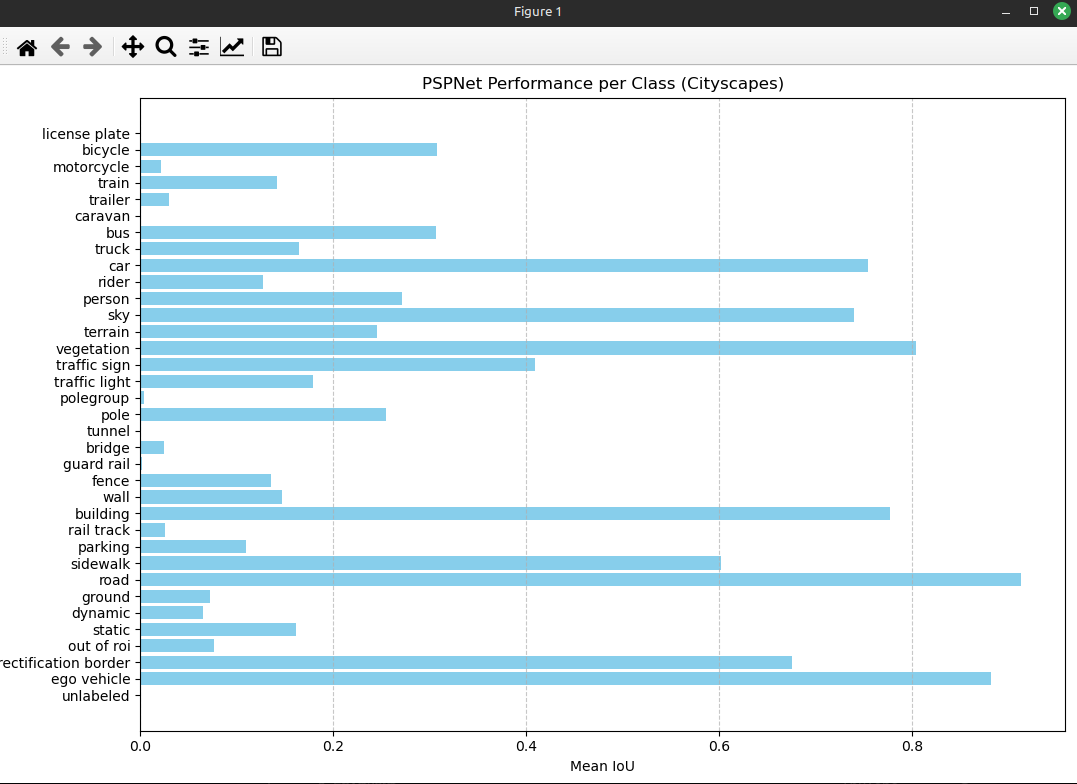
\includegraphics[width=0.6\textwidth]{barplot.png}
    \caption{Mean IoU ανά κλάση}
    \end{figure}


\paragraph{Ground Truth vs Prediction}
\mbox{}\\
\begin{enumerate}
    \item \textbf{Σωστή Ταξινόμηση Αντικειμένων:} Το μοντέλο αναγνωρίζει σωστά τη σημασιολογική κατηγορία των αντικειμένων, για παράδειγμα διακρίνοντας αποτελεσματικά πχ τη \textit{Vegetation} από το \textit{Building}.

    \item \textbf{Ποιότητα Εντοπισμού (Localization):} Τα όρια στην πρόβλεψη εμφανίζονται θολά σε σύγκριση με τις κοφτερές ακμές στο \textit{ground truth}. Το φαινόμενο αυτό δείχνει ότι, παρότι το μοντέλο προσδιορίζει σωστά το \textit{τι} είναι το αντικείμενο, η διαδικασία \textit{downsampling/upsampling} περιορίζει την ικανότητά του να εντοπίσει με ακρίβεια το \textit{πού} βρίσκονται οι ακμές.
\end{enumerate}


\begin{figure}[h!]
    \centering
    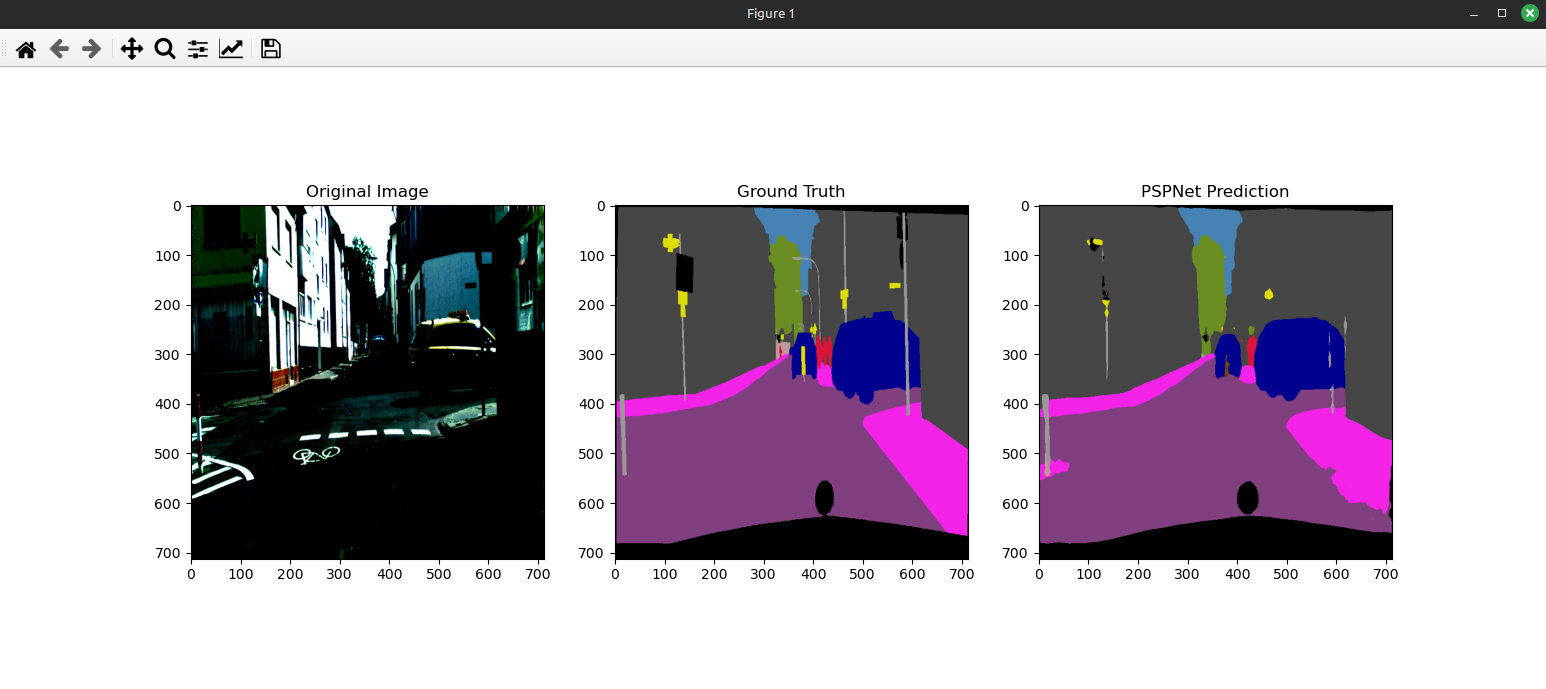
\includegraphics[width=0.7\textwidth]{prediction.png}
    \caption{Prediction vs Ground Truth}
    \end{figure}








\end{document}